\documentclass[
11pt,%
tightenlines,%
twoside,%
onecolumn,%
nofloats,%
nobibnotes,%
nofootinbib,%
superscriptaddress,%
noshowpacs,%
centertags]%
{revtex4}
\usepackage{ljm}
\usepackage{listings}
\usepackage[utf8]{inputenc}
\usepackage[russian]{babel}

\lstset{
language=C++,
basewidth=0.5em,
xleftmargin=45pt,
xrightmargin=45pt,
basicstyle=\small\ttfamily,
keywordstyle=\bfseries\underbar,
numbers=left,
numberstyle=\tiny,
stepnumber=1,
numbersep=10pt,
showspaces=false,
showstringspaces=false,
showtabs=false,
frame=trBL,
tabsize=2,
captionpos=t,
breaklines=true,
breakatwhitespace=false,
escapeinside={\%*}{*)}
}

\begin{document}

\titlerunning{Computational mesh evolution}
\authorrunning{Meshcheryakov et al.}

\title{Evolution of the surface computational mesh in the ice accretion process}

\author{\firstname{A.~O.}~\surname{Meshcheryakov}}
\email[E-mail: ]{alex2501@jscc.ru}
\affiliation{Joint Supercomputer Center of the Russian Academy of Sciences -- branch of Scientific Research Institute of System Analysis of the Russian Academy of Sciences, Leninsky prospect 32a, Moscow, 119334, Russia}

\author{\firstname{A.~A.}~\surname{Rybakov}}
\email[E-mail: ]{rybakov@jscc.ru}
\affiliation{Joint Supercomputer Center of the Russian Academy of Sciences -- branch of Scientific Research Institute of System Analysis of the Russian Academy of Sciences, Leninsky prospect 32a, Moscow, 119334, Russia}

\firstcollaboration{(Submitted by TODO)} % Add if you know submitter.
%\lastcollaboration{ }

\received{TODO}

\begin{abstract}
%Задача моделирования обледенения поверхности обтекаемого тела является критической для обеспечения безопасности полетов в условия ледообразования.
The task of modeling the ice accretion of the surface of a streamlined body is critical for ensuring flight safety in conditions of ice formation.
%Формирование ледяных наростов на несущих частях и элементах силовых установок летальных аппаратов может существенно влиять на летные характеристики.
The formation of ice growths on the bearing parts and elements of the power systems of aircraft can significantly affect the flight characteristics.
%Сам процесс ледообразования является комплексным.
The process of ice formation itself is complex.
%Для получения качественной картины профиля ледяного нароста необходимо учитывать множество физических процессов, включая динамику газа, теплопроводность, динамику капель, выпадающих на поверхность, течение жидкости по поверхности.
To obtain a qualitative picture of the ice buildup profile, it is necessary to take into account many physical processes, including gas dynamics, thermal conductivity, the dynamics of drops falling to the surface, and the flow of liquid over the surface.
%Расчет ледяного покрова должен выполняться итерационно, так как образующийся лед существенно влияет на газодинамические характеристики, которые должны пересчитываться с ростом льда.
The calculation of the ice cover must be performed iteratively, since the resulting ice significantly affects the gas-dynamic characteristics, which must be recalculated with ice growth.
%Важной частью моделирования является эволюция поверхности тела в процессе ледообразования.
An important part of modeling is the evolution of the ice surface in the process of ice formation.
%В настоящей статье рассматриваются различные подходы к моделированию эволюции поверхности, предлагается новый алгоритм построения новой поверхности с помощью общей огибающей семейства сфер, центры которых находятся на исходной поверхности.
This article discusses various approaches to modeling the evolution of a surface and proposes a new algorithm for constructing a new surface using a common envelope of a family of spheres whose centers are located on the original surface.
%В процессе эволюции на поверхности могут образовываться различные артефакты и аномалии, из-за которых проведение дальнейших расчетов может стать невозможным.
In the process of evolution, various artifacts and anomalies may form on the surface, due to which further calculations may become impossible.
%Для устранения этих препятствий в статье рассматриваются методы адаптации расчетной сетки в процессе эволюции, а также устранения потенциальных самопересечений, препятствующих дальнейшим расчетам.
To eliminate these obstacles, the article considers methods for adapting the computational mesh in the process of evolution, as well as eliminating potential self-intersections that impede further calculations.
\end{abstract}

%\subclass{TODO subclass} % Enter 2010 Mathematics Subject Classification.

\keywords{Ice formation, unstructured surface computational mesh, surface evolution.}

\maketitle

%---------------------------------------------------------------------------------------------------

\section{Introduction}

%Численное моделирование процесса обледенения поверхности тела является сложной мультифизичной задачей, включающей в себя моделирование процессов газовой динамики, теплообмена, течения жидкости, динамики капель в воздушном потоке и других.
Numerical simulation of the body surface icing process is a complex multiphysics problem, which includes modeling the processes of gas dynamics, heat transfer, fluid flow, droplet dynamics in an air flow, and others.
%Исследование процессов ледообразования имеет важное практическое значение.
The study of ice formation processes is of great practical importance.
%В частности характер и интенсивность образования льда на поверхности летательного аппарата критическим образом влияет на его летные характеристики, что напрямую связано с безопасностью полетов \cite{Raj}.
In particular, the nature and intensity of ice formation on the surface of an aircraft critically affects its flight characteristics, which is directly related to flight safety \cite{Raj}.

%На сегодняшний день среди зарубежного программного обеспечения для моделирования процесса ледообразования лидером является программный комплекс ANSYS (включая модули FENSAP-ICE, DROP3D, ICE3D) \cite{Martini}.
Today, among foreign software for modeling the process of ice formation, the leader is the ANSYS software package (including modules FENSAP-ICE, DROP3D, ICE3D) \cite{Martini}.
%В России также активно ведется разработка математических алгоритмов и программного обеспечения по этому направлению.
In Russia there are also a lot of mathematical algorithms and software in this area beeing actively developed.
%Можно отметить исследования по разработке модуля iceFoam в составе открытого пакета OpenFOAM~\cite{Strijhak}.
We can note the research on the development of the iceFoam module as part of the open source package OpenFOAM~\cite{Strijhak}.
%Среди коммерческих продуктов в последние годы активно развивается пакет IceVision в составе программного комплекса FlowVision~\cite{Sorokin}, а также решение в составе пакета инженерного анализа ЛОГОС \cite{Galanov}.
Among commercial products, the IceVision package has been actively developed in recent years as part of the FlowVision~\cite{Sorokin} software package, and a solution as part of the LOGOS \cite{Galanov} engineering analysis package.

%Моделирование процесса ледяного покрова осуществляется, как правило, на поверхностной расчетной сетке и состоит из двух основных частей.
Modeling of the ice cover process is carried out, as a rule, on a surface computational mesh and consists of two main parts.
%Первой частью является вычисление интенсивности нарастания льда в отдельных элементах сетки (это может быть вычисление массы скопившегося льда в каждой ячейке расчетной сетки за единицу времени, либо скорость образования ледяного покрова в узлах сетки, либо другие аналогичные характеристики).
The first part is the calculation of the intensity of ice growth in individual mesh elements (this can be the calculation of the mass of accumulated ice in each face of the computational mesh per unit of time, or the rate of ice cover formation at the grid nodes, or other similar characteristics).
%Для выполнения вычисления интенсивности нарастания льда в элементах расчетной сетки существует множество моделей ледообразования \cite{Bartkus,Zhang,Pena}, учитывающих разные состояния льда, динамику водяной пленки, тепловые потоки и другие факторы.
To calculate the intensity of ice growth in the elements of the computational mesh, there are many models of ice formation \cite{Bartkus,Zhang,Pena} that take into account different states of ice, water film dynamics, heat fluxes, and other factors.
%Модели ледообразования не рассматриваются в рамках данной работы.
Ice formation models are not considered within the scope of this paper.
%Второй важной составляющей моделирования ледяного нароста является определение изменения поверхности тела после нарастания на ней слоя льда.
The second important component of ice build-up modeling is the determination of changes in the body surface after the growth of an ice layer on it.
%В данной статье рассматриваются наиболее известные подходы к моделированию эволюции поверхности обледеневающего тела, а также предлагается новый алгоритм эволюции поверхности, основанный на принципе общей огибающей семейства сфер, центры которых лежат на исходной поверхности, и алгоритм устранения самопересечений сетки, которые могут возникать из-за изменения положения узлов в процессе эволюции.
This article discusses the most well-known approaches to modeling the evolution of the surface of an icing body, and also proposes a new surface evolution algorithm based on the principle of a common envelope of a family of spheres whose centers lie on the original surface, and an algorithm for eliminating mesh self-intersections that may occur due to changes in positions of nodes in the process of evolution.

%---------------------------------------------------------------------------------------------------

\section{Mesh architecture}

Решение задачи перестроения поверхности будем рассматривать на неструктурированной поверхностной расчетной сетке.
Элементами расчетной сетки являются узлы ($N$), ребра ($e$)  и ячейки ($f$).
Для удобства каждый элемент сетки связан со всеми своими инцидентными элементами: так связаны между собой инцидентные узлы и ребра, узлы и ячейки, ребра и ячейки. Множество инцидентных узлов будем обозначать $\mathscr{N}$, множество инцидентных ребер будем обозначать $\mathscr{E}$, а множество инцидентных ячеек будем обозначать $\mathscr{F}$.

\begin{figure}[h]
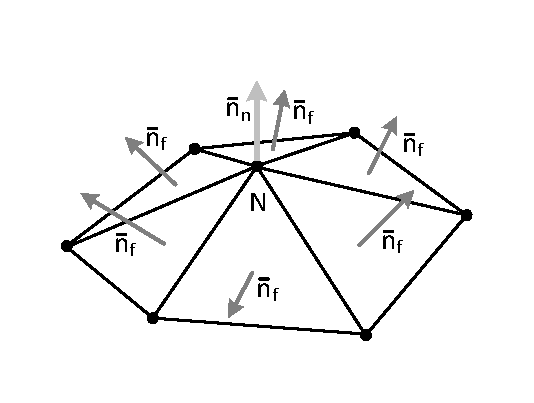
\includegraphics[width=0.48\textwidth]{pics/pic_architecture_size.pdf}
\captionstyle{center}\caption{Архитектура расчетной сетки.}\label{fig:pic_architecture}
\end{figure}

К расчетной сетке предъявляются следующие требования.
Во-первых, сетка должна быть целостной, то есть каждое ребро имеет ровно два инцидентных узла, отсутствуют изолированные и висячие узлы, а также изолированные ребра.
Во-вторых, все ячейки должны представлять собой треугольники (это гарантирует, что ячейка является плоской, так как четыре и более произвольных узлов могут не лежать в одной плоскости).
И в-третьих, рассматриваются только замкнутые сетки, представляющие собой поверхности, то есть каждое ребро имеет ровно две инцидентные ячейки.

\begin{equation}\label{eq_arch}
\begin{cases}
\forall N \Rightarrow \mathscr{E}(N) > 2, \mathscr{F}(N) > 2 \\
\forall e \Rightarrow \mathscr{N}(e) = 2 , \mathscr{F}(e) = 2 \\
\forall f \Rightarrow \mathscr{N}(f) = 3 , \mathscr{E}(f) = 3 \\
\end{cases}
\end{equation}

В качестве дополнения также будем требовать, чтобы сетка представляла собой двустороннюю поверхность, для каждой ячейки однозначно определена нормаль к поверхности $\vec{n}_f$.
Также никакие два узла сетки не совпадают и отсутствуют ячейки с нулевой площадью (так как это сделает невозможным вычислений нормалей).
Для узла сетки будем рассматривать понятие нормали к поверхности и определять эту нормаль как

\begin{equation}
\vec{n}_n(N) = \frac{1}{|\mathscr{F}(N)|} \sum_{f \in \mathscr{F}(N)}{\vec{n}_f(f)}
\end{equation}

%---------------------------------------------------------------------------------------------------

\section{Remeshing}

Центральная задача перестроения поверхности из-за нарастания ледяного покрова выглядит следующим образом.
Пусть известно, что в результате численного решения задачи ледообразования конечно-объемным методом \cite{Beaugendre} в каждой ячейке сетки была вычислена масса накопленного льда ($m$).
Будем считать плотность льда постоянной, то есть в каждой ячейке также известен объем накопленного льда ($V$).
Для каждого узла сетки $N$ требуется найти его новое положение в пространстве $N'$, чтобы для каждой ячейки с узлами $ABC$ объем пространства, ограниченный фигурой $ABCA'B'C'$ соответствовал объему льда, накопленному в данной ячейке.

Следует отметить, что поставленная задача может не иметь точного решения, и в этом случае следует стремиться к минимизации ошибки по объему (когда фактически образовавшийся объем льда не слишком сильно отличается от целевого объема, то есть разница $V_{ABCA'B'C'} - V$ мала).

Задачу определения новых положений узлов расчетной сетки можно разделить на две задачи: определение направлений смещения узлов и определение величин смещения.
Далее рассмотрим отдельные методы перестроения поверхностей более подробно.

\subsection{Classical remeshing methods}

Простейшие классические методы перестроения выполняются в предположении, что направление смещения узла совпадает с нормалью, проведенной из этого узла.
Таким образом, необходимо лишь определить величину смещения.
Отметим, что в двумерной постановке можно найти оптимальное решение (обеспечивающее минимальное отклонение по объему от целевого значения) поставленной задачи \cite{Rybakov_2D}.

\begin{figure}[h]
  \centering
  \begin{minipage}[h]{0.49\textwidth}
    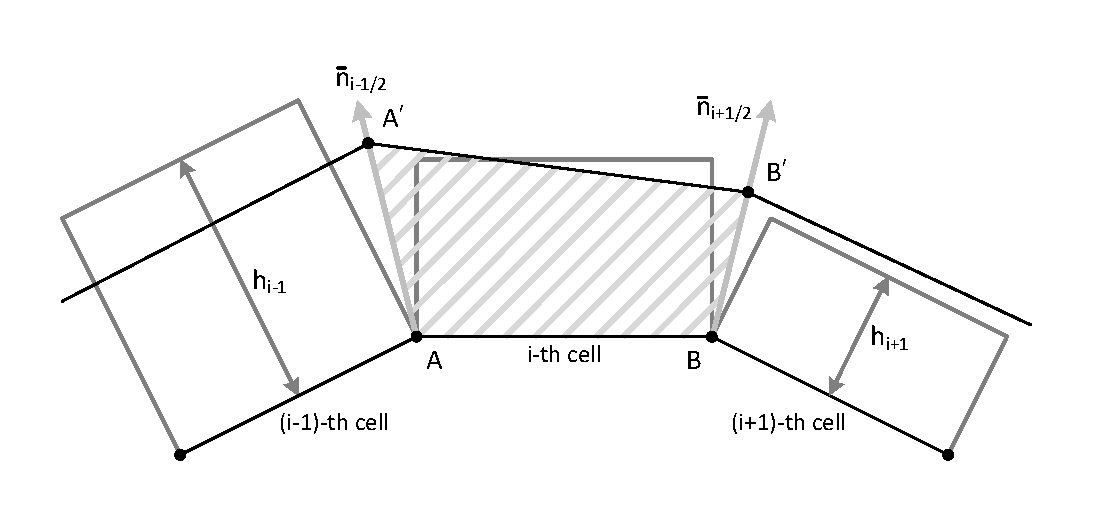
\includegraphics[width=\textwidth]{pics/pic_classical_methods_rectangles_size.pdf}
    \caption{Перестроение поверхности с помощью метода прямоугольников в 2D.}\label{fig:pic_classical_methods_rectangles}
  \end{minipage}
  \hfill
  \begin{minipage}[h]{0.49\textwidth}
    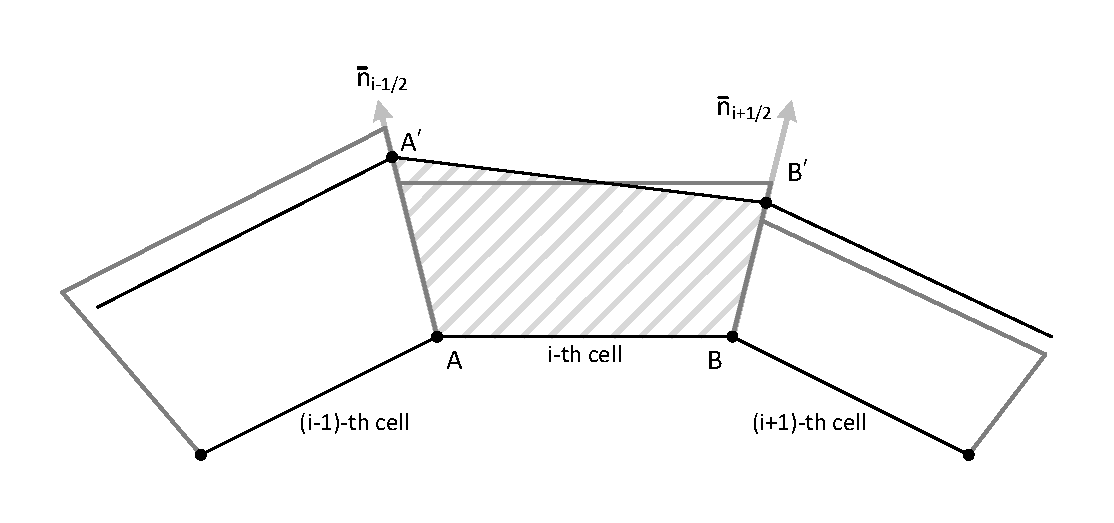
\includegraphics[width=\textwidth]{pics/pic_classical_methods_trapezoids_size.pdf}
    \caption{Перестроение поверхности с помощью метода трапеций в 2D.}\label{fig:pic_classical_methods_trapezoids}
  \end{minipage}
\end{figure}

В качестве первого метода рассмотрим метод призм (в двумерной постановке аналогом данного метода является метод прямоугольников, продемонстрированный на Fig.~\ref{fig:pic_classical_methods_rectangles}).
В этом методе входными данными является объем накопленного льда в каждой ячейке сетки ($V(f)$).
На первым шаге в каждой ячейке ищется толщина ледяного покрова в предположении, что лед в пределах одной ячейки имеет форму призмы, и ячейка является основанием этой призмы.
Тогда толщина ледяного покрова равняется $h(f) = \frac{V(f)}{S(f)}$, где $S(f)$ -- площадь ячейки.
После чего величина смещения каждого узла вычисляется просто как среднее арифметическое высот ледяного покрова во всех инцидентных ячейках:

\begin{equation}
h(N) = \frac{1}{|\mathscr{F}(N)|} \sum_{f \in \mathscr{F}(N)}{h(f)}
\end{equation}

Второй метод можно назвать методом пирамид (в двумерной постановке аналогом данного метод является метод трапеций, показанный на Fig.~\ref{fig:pic_classical_methods_trapezoids}).
Входными данными также является объем накопленного льда в каждой ячейке сетки ($V(f)$).
Однако в отличие от предыдущего метода объем накопленного в ячейке льда представляется не призмой, а усеченной пирамидой, основанием которой является ячейка, а боковые ребра направлены вдоль нормалей узлов.
Высота этой усеченной пирамиды ищется из соотношения $V(f) = \frac{1}{3} h (2S + hS'_h + \sqrt{S(S + hS'_h)})$, где величина $S'_h$ определяется направлениями нормалей узлов ячейки.
Тогда как узлы ячейки являются точками первого основания построенной пирамиды, точки второго основания представляют собой новые положения узлов, вычисленных относительно рассматриваемой ячейки.
Таким образом, у каждого узла сетки вычисляется несколько новых положений (каждое из которых вычислено относительно своей инцидентной ячейки).
Для двумерного случая получается ровно два таких новых положения (так как в двумерном случае каждый узел имеет ровно две инцидентные ячейки), для трехмерного случае таких точек более двух.
Для выбора единственного нового положения узла сетки берется среднее значение из всех положений, вычисленных относительно инцидентных ячеек.

Из рассмотренных двух методов интуитивно создается впечатление, что метод пирамид должен быть более точным, так как он учитывает потери и избыток объема льда, образующиеся из-за изломов сетки (так как соседние ячейки не лежат в одной плоскости, то представление льда в ячейках в виде призм неизбежно приводит к образованию пробелов или наложений частей льда в виде призм друг на друга).
Но по крайней мере в двумерном случае это предположение оказывается неверным, так как метод прямоугольников демонстрирует меньшее отклонение от точного решения по сравнению с методом трапеций \cite{Rybakov_2D}.

\begin{figure}[h]
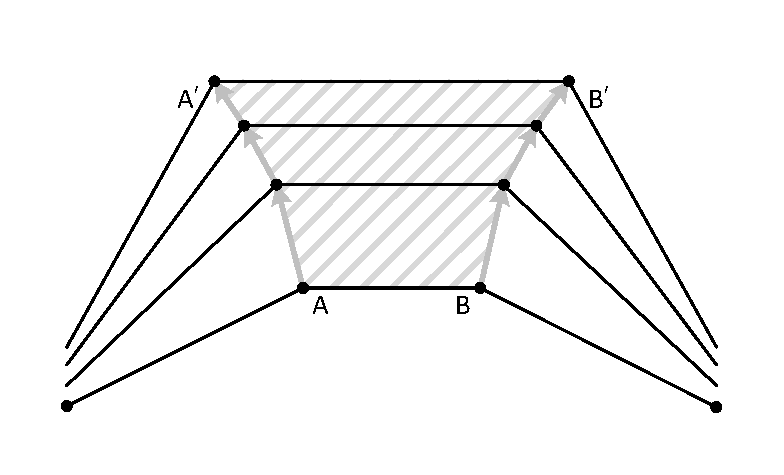
\includegraphics[width=0.48\textwidth]{pics/pic_classical_methods_multilayer_size.pdf}
\captionstyle{center}\caption{Многослойное перестроение сетки.}\label{fig:pic_classical_methods_multilayer}
\end{figure}

Вне зависимости от используемого метода перестроения значительно повысить точность можно с помощью многослойного подхода \cite{BourgaultCote}.
В этом случае вместо однократного перестроения сетки по объему накопленного льда в каждой ячейке ($V(f)$), выбирается фиксированное количество шагов перестроения $k$, а дальше процедура выполняется $k$ раз подряд, но с использованием объема накопленного в ячейке льда $\frac{V(f)}{k}$.
Точность повышается из-за того, что после каждого шага перестроения нормали в узлах сетки меняют свое направление, и общий объем наращиваемого льда становится более криволинейным, лучше учитывает геометрию сетки и, как следствие, точнее соответствует исходному значению $V(f)$ (см. Fig.~\ref{fig:pic_classical_methods_multilayer}).

\subsection{Перестроение сохранением объема}

%В работах \cite{Thompson,Tong} описан устойчивый итерационный алгоритм эволюции поверхностной сетки, сохраняющий целевой объем льда.
The articles \cite{Thompson,Tong} describe a stable iterative grid evolution algorithm that preserves the target volume of ice.
%В нем используется ряд улучшений по сравнению с классическими методами.
It uses several improvements over the classical methods.

%Многослойный подход, реализованный в этом методе, не использует константное количество шагов - величина наращиваемого объема на каждом шаге алгоритма рассчитывается исходя из максимально допустимой доли временного шага обледенения, после превышения которого возможно развитие численной нестабильности в эволюции поверхности.
The multilayer approach implemented in this method does not use a constant number of steps - the value of the increased volume at each step of the algorithm is calculated based on the maximum allowable fraction of the icing time step, after exceeding which numerical instability may occur in the evolution of the surface.
%Наиболее очевидный случай возникает, когда проекции нормалей граней пересекаются, в этом случае слишком большой временной шаг приведет к складыванию поверхности.
The most obvious case occurs when the face normal projections intersect, in which case too large a time step will cause the surface to fold.
%Чтобы идентифицировать грани, которые будут демонстрировать подобное поведение на текущем временном шаге, предполагается, что объем, образованный путем вытягивания треугольной грани с использованием параллельной плоскости смещения, образует призматоид, объем которого определяется кубической функцией высоты $h$:
In order to identify faces that will exhibit such behavior at the current time step, it is assumed that the volume formed by extruding a triangular face using a parallel displacement plane forms a prismatoid whose volume is given by the cubic function of the height $h$:

\begin{equation}\label{Tong:1}
V(h)=ah+bh^2+ch^3
\end{equation}

%где константы $a$, $b$, $c$ определяются позициями узлов грани, их нормалей и нормалью грани.
where the constants $a$, $b$, $c$ are determined by the positions of the face nodes, their normals, and the face normal.
%Рассмотрим корни квадратного уравнения, которое получается в результате дифференцирования уравнения \ref{Tong:1}.
Consider the roots of the quadratic equation, which is obtained as a result of differentiation of the equation \ref{Tong:1}.
%Если корни являются положительными вещественными значениями, наименьший положительный корень определяет высоту, на которой достигается максимальный объем, которая обозначается как $V_{max}$, иначе функция монотонна с возрастанием и ограничение на шаг в данной грани не требуется.
If the roots are positive real values, the smallest positive root determines the height at which the maximum volume is reached, which is denoted as $V_{max}$, otherwise the function is monotonic with increasing and no step restriction is required in this face.
%Исходя из этого, можно вычислить максимальную долю временного шага обледенения, которая требуется для обеспечения разумного поведения накопления объема.
From this, it is possible to calculate the maximum fraction of the icing time step that is required to ensure reasonable volume accumulation behavior.
%В дополнение к этому пределу размера шага был введен предел стабильности $\alpha_{jiao}$, который основан на том, как изменяются направления нормалей по мере эволюции поверхности \cite{Jiao}.
In addition to this step size limit, a $\alpha_{jiao}$ stability limit has been introduced, which is based on how normal directions change as the surface evolves \cite{Jiao}.
%Тогда, допустимая доля временного шага для $i$-й грани определяется как
Then, the allowable fraction of the time step for the $i$-th face is defined as

\begin{equation}\label{Tong:2}
\alpha_{\Delta t}^i=
\begin{cases}
min(s_{\Delta t}\frac{V_{max}^i}{V_f},\alpha_{jiao},1), \text{if $V_{max}^i$ exists}, \\
\alpha_{jiao}, \text{if $V_{max}^i$ doesn't exist}
\end{cases}
\end{equation}

%где $s_{\Delta t}$ ($0 < s_{\Delta t} < 1$) -- эмпирически определяемый коэффициент, $V_f$ -- текущий оставшийся объем приращения льда для $i$-й грани.
where $s_{\Delta t}$ ($0 < s_{\Delta t} < 1$) is an empirically determined coefficient, $V_f$ is the current remaining ice increment volume for the $i$-th face.
%Тогда объем, наращенный для текущего шага, равен $\alpha_{\Delta t} V_f$, где $\alpha_{\Delta t}$ представляет собой глобальное минимальное значение для всех граней.
Then the volume built up for the current step is $\alpha_{\Delta t} V_f$, where $\alpha_{\Delta t}$ is the global minimum value for all faces.

%Другой важной особенностью алгоритма является введение первичного и нулевого простанств, описанных в \cite{Jiao_null_space_smooth}.
Another important feature of the algorithm is the introduction of primary and null spaces, described in \cite{Jiao_null_space_smooth}.
%Если эволюционное движение узлов сетки происходит в первичном пространстве, то их перемещение в нулевом пространстве будет сохранять потенциальную точность второго порядка триангуляции поверхности, благодаря чему мы можем  проводить сглаживание поверхности сетки с сохранением объема.
If the evolutionary movement of mesh nodes occurs in primary space, then their movement in zero space will preserve the potential accuracy of the second order of triangulation of the surface, so that we can maintain volume when smoothing the mesh surface.
%В алгоритме используется несколько видов сглаживаний.
The algorithm uses several types of smoothing.

%Первое сглаживание -- сглаживание нормалей в вершинах и ячейках сетки.
The first smoothing is the smoothing of the normals in the mesh nodes and faces.
%Чтобы сделать возможным сглаживание в нулевом пространстве, все нормали в узлах рассчитываются так, чтобы они лежали в первичном пространстве, а перемещение узлов при наращивании льда происходит только по их нормалям.
To make smoothing possible in zero space, all normals at nodes are calculated so that they lie in primary space, and the movement of nodes during ice buildup occurs only along their normals.
%По мере эволюции, на поверхности может усиливаться шум -- если его не контролировать, может возникнуть ситуация, когда двугранный угол между гранями станет слишком малым и ограничит максимальную долю временного шага обледенения.
As evolution progresses, surface noise can increase - if left unchecked, a situation can arise where the dihedral angle between the faces becomes too small and limits the maximum fraction of the icing time step.
%Для уменьшения поверхностного шума, перед наращиванием льда применяется локальное сглаживание, регулирующее направление смещения узла в проблемных областях, чтобы оно более точно совпадало с направлениями его соседей.
To reduce surface noise, local smoothing is applied before ice builds up, adjusting the direction of node displacement in problem areas so that it more closely matches the directions of its neighbors.
%Этот метод может улучшить гладкость поверхности в некоторых ситуациях.
This method can improve surface smoothness in some situations.
%Основная цель сглаживания нормалей -— вытолкнуть точки из вогнутых областей, где нормали могут локально сходиться.
The main purpose of normal smoothing is to push points out of concave areas where normals can converge locally.
%Сглаживание нормалей достигается с помощью серий взвешенных средних, которые предназначены для придания веса нормалям, генерируемым проблемными областями.
Normal smoothing is achieved using a series of weighted averages, which are designed to give weight to the normals generated by problem areas.

%Второе сглаживание -- сглаживание высот.
The second smoothing is height smoothing.
%После вычисления доли временного шага и объема, наращиваемого для текущего шага, для эволюции поверхности необходимо определить поле высот, которое будет соответствовать этому объему, чтобы по нему определить смещения узлов сетки.
After calculating the fraction of the time step and the volume that is increased for the current step, it is necessary to determine the height field for the evolution of the surface , which will correspond to this volume, in order to determine the offsets of the grid nodes from it.
%Решение $V(h_i) = \alpha_{\Delta t} V_f$ обеспечивает поле начальных высот, которое используется для движения поверхности.
The solution $V(h_i) = \alpha_{\Delta t} V_f$ provides the initial height field that is used to move the surface.
%Цель дополнительного шага сглаживания высоты состоит в том, чтобы отфильтровать высокочастотный шум в поле высот за счет уменьшения разницы высот между соседними гранями.
The purpose of the additional height smoothing step is to filter out high-frequency noise in the height field by reducing the difference in height between adjacent faces.
%Как правило, высоты двух треугольных граней, имеющих общее ребро, не будут равными.
Usually, the heights of two triangular faces that share a common edge will not be equal.
%На данном шаге используется сглаживание высот с сохранением объема путем его перераспределения между соседними гранями.
At this step, smoothing of heights is used while preserving the volume by redistributing it between adjacent faces.

\begin{figure}
  \centering
  \begin{minipage}[h]{0.49\textwidth}
    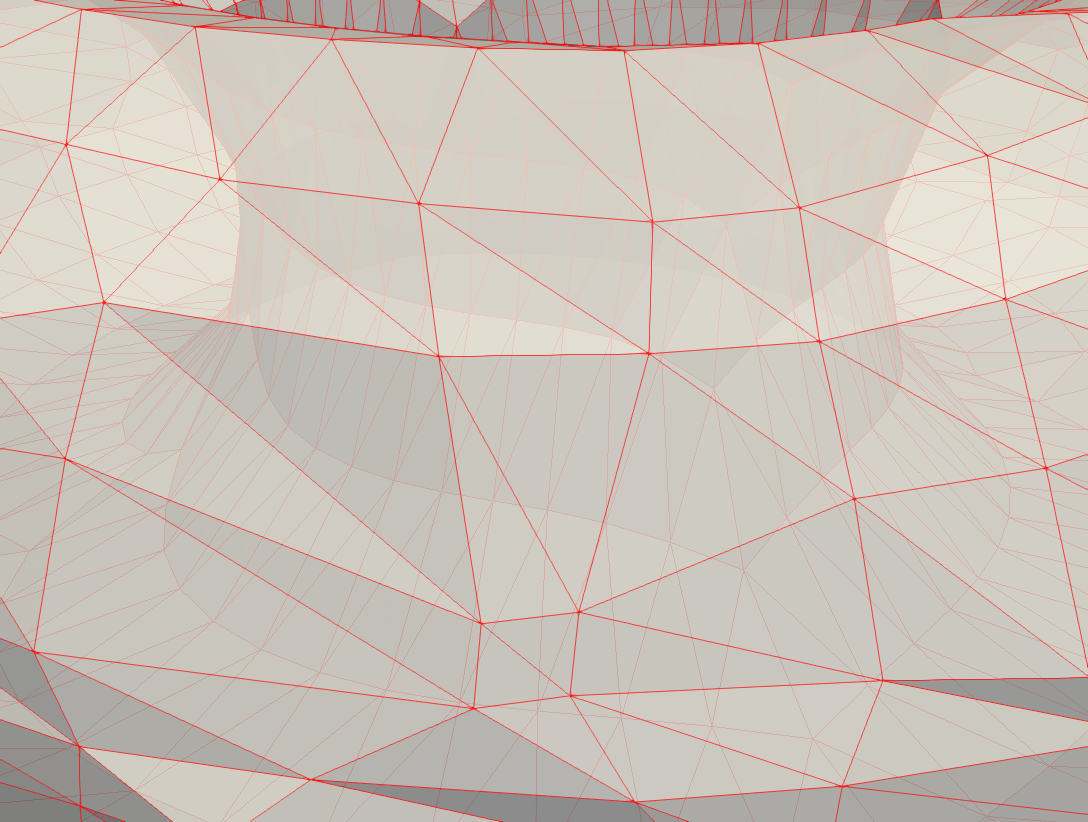
\includegraphics[width=\textwidth]{pics/pic_smooth_before.png}
    \caption{Mesh before null-space smoothing}\label{fig:pic_smooth_before}
  \end{minipage}
  \hfill
  \begin{minipage}[h]{0.49\textwidth}
    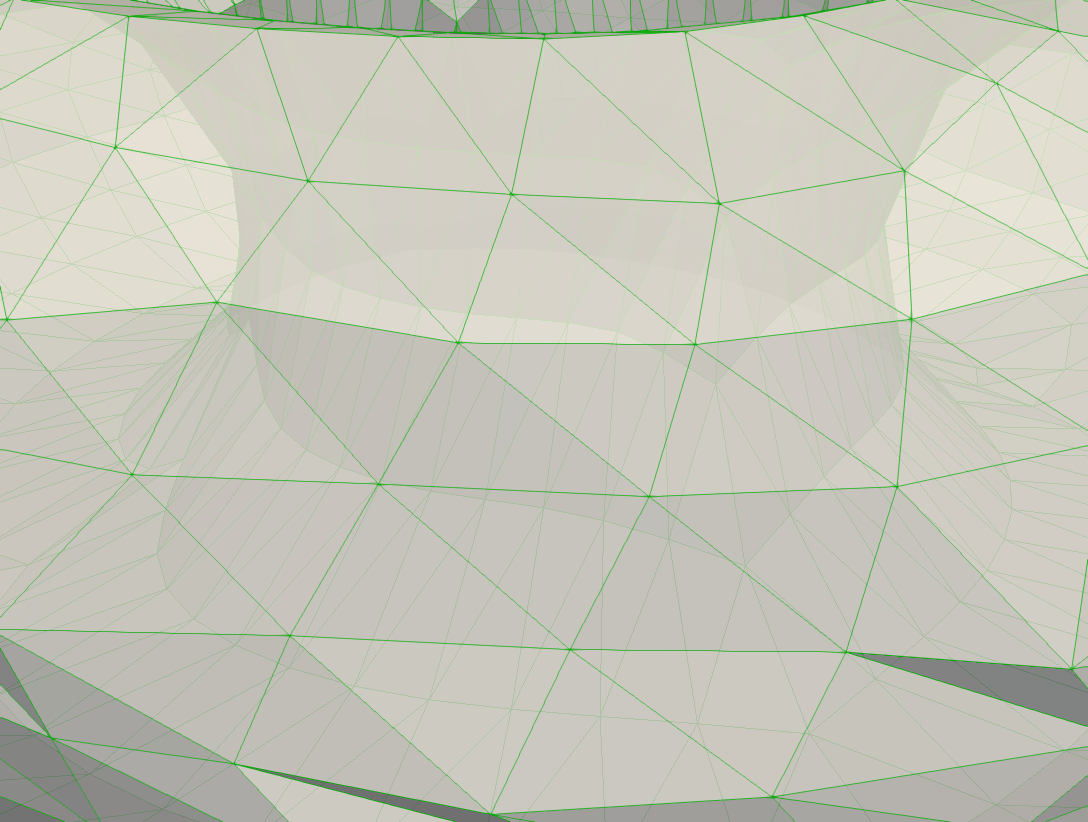
\includegraphics[width=\textwidth]{pics/pic_smooth_after.png}
    \caption{Mesh after null-space smoothing.}\label{fig:pic_smooth_after}
  \end{minipage}
\end{figure}

%Последним типом сглаживания является сглаживание в нулевом пространстве.
The last type of smoothing is null space smoothing.
%Эволюция поверхности будет стремиться упаковать узлы в вогнутые области, где сходятся нормали к поверхности, тогда как расширение сетки происходит в выпуклых областях, где нормали к поверхности расходятся.
Surface evolution will tend to pack nodes into concave regions where surface normals converge, while mesh expansion occurs in convex regions where surface normals diverge.
%Если узлы не будут перераспределены, может стать невозможным продолжать продуктивный, стабильный временной шаг.
If the nodes are not reallocated, it may become impossible to continue with a productive and stable time step.
%Для улучшения качества поверхностной сетки узлы перераспределяются на поверхности с помощью сглаживания в нулевом пространстве.
To improve the quality of the surface mesh, the nodes are redistributed on the surface using null space smoothing.
%Этот метод способен перераспределять точки, сохраняя при этом целостность базовой геометрии.
This method is able to redistribute points while maintaining the integrity of the base geometry.
%Нулевое пространство определяется касательной плоскостью (для гладких областей), касательной линией (для складок поверхности) или пустым пространством (для углов), движущиеся в нем узлы остаются на поверхности, так что объем и форма поверхности могут быть сохранены (Fig.~\ref{fig:pic_smooth_before}, Fig.~\ref{fig:pic_smooth_after}).
Null space is defined by a tangent plane (for smooth areas), a tangent line (for surface wrinkles), or empty space (for corners), nodes moving in it remain on the surface, so that the volume and shape of the surface can be preserved (Fig.~\ref{fig:pic_smooth_before}, Fig.~\ref{fig:pic_smooth_after}).

\subsection{Метод общей огибающей}

Рассмотрим задачу определения новых положений узлов расчетной сетки немного в другой постановке.
Пусть для каждого узла $\vec{N}$ известна линейная скорость нарастания льда $v(\vec{N})$ (в метрах в секунду).
Будем считать, что нарастание льда в любой точке роста выполняется одновременно во всех направлениях аналогично принципу Гюйгенса-Френеля распространения волн.
Тогда фронт распространения льда от произвольной точки $\vec{P}$ через промежуток времени $\Delta t$ будет иметь форму сферы с центром в точке $\vec{P}$ и радиусом $v(\vec{P}) \Delta t$.
Далее будем предполагать, что выполняется расчет новых положений узлов через некоторый фиксированный момент времени $\Delta t$, то есть для каждого узла известен радиус продвижения фронта льда $R(\vec{N}) = v(\vec{N}) \Delta t$.
Так как элементами расчетной сетки являются треугольники, то необходимо определить радиус продвижения фронта льда для каждой внутренней точки треугольника по данным его вершин.

Рассмотрим ячейку расчетной сетки, вершинами которой являются точки $\vec{A}$, $\vec{B}$, $\vec{C}$.
Точки треугольника представляют собой геометрическое место точек, описываемое следующим образом:

\begin{equation}
\begin{cases}
\vec{P}(\beta, \gamma) = \vec{A} + \beta (\vec{B} - \vec{A}) + \gamma (\vec{C} - \vec{A}) = \vec{A} + \beta \vec{AB} + \gamma \vec{AC} \\
\beta \ge 0 \\
\gamma \ge 0 \\
\beta + \gamma \le 1
\end{cases}
\end{equation}

Определим для каждой точки треугольника $\vec{P}(\beta, \gamma)$ радиус продвижения фронта льда как $R(\vec{P}(\beta, \gamma)) = R(\beta, \gamma) = R(\vec{A}) + \beta (R(\vec{B}) - R(\vec{A})) + \gamma (R(\vec{C}) - R(\vec{A})) = R_A + \beta R_{AB} + \gamma R_{AC}$.
Фронт продвижения льда от точки $\vec{P}(\beta, \gamma)$ представляет собой сферу $S(\beta, \gamma) = S(\vec{P}(\beta, \gamma), R(\beta, \gamma))$.
Фронтом продвижения льда всей треугольной ячейки будем считать общую огибающую сфер, построенных на всех точках этой ячейки, что показано на Fig.~\ref{fig:pic_general_envelope_size}.

\begin{figure}
  \centering
  \begin{minipage}[b]{0.48\textwidth}
    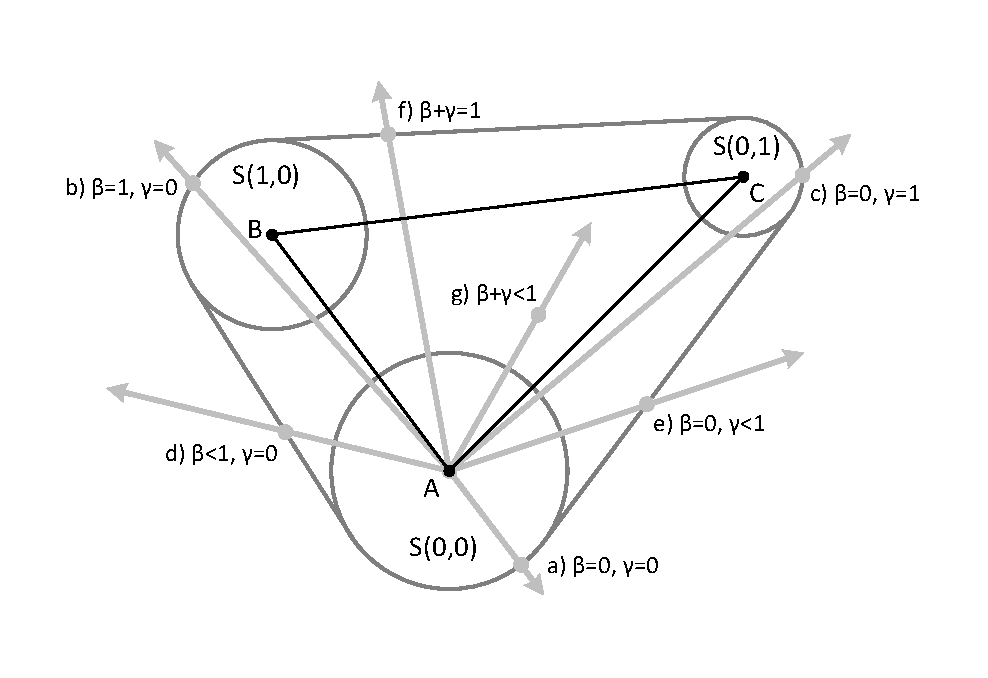
\includegraphics[width=\textwidth]{pics/pic_general_envelope_size.pdf}
    \caption{Общая огибающая поверхность сфер, построенных на точках треугольника.}\label{fig:pic_general_envelope_size}
  \end{minipage}
  \hfill
  \begin{minipage}[b]{0.48\textwidth}
    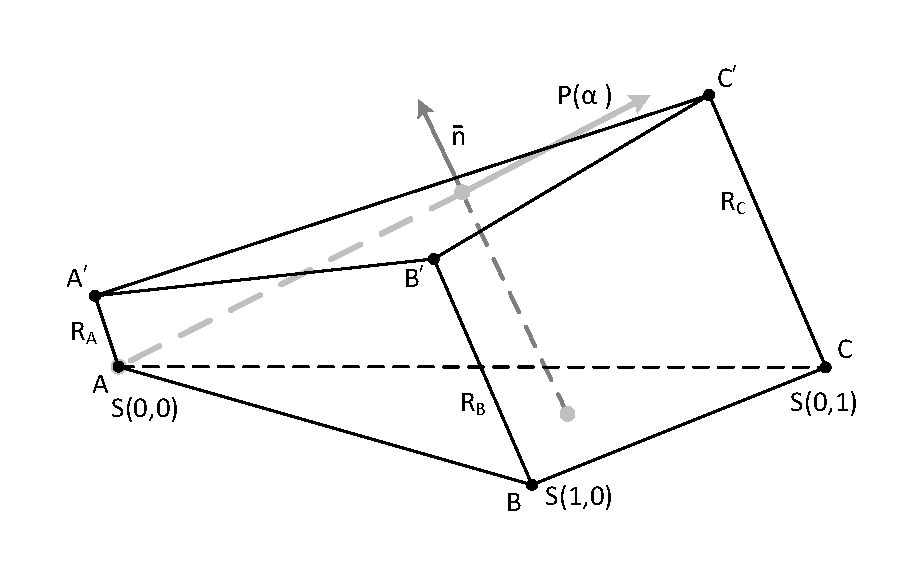
\includegraphics[width=\textwidth]{pics/pic_general_envelope_2_size.pdf}
    \caption{Поиск нового положения узла на общей касательной плосткости трех сфер.}\label{fig:pic_general_envelope_2_size}
  \end{minipage}
\end{figure}

При изменении положения узлов расчетной сетки (точки $\vec{A}$, $\vec{B}$, $\vec{C}$) будем исходить из предположения, что после перемещения узлы будут находиться на общей огибающей поверхности множества сфер $S(\beta, \gamma)$ (новые положения узлов -- точки $\vec{A'}$, $\vec{B'}$, $\vec{C'}$).
Пока в расчете не учитываем влияние соседних расчетных ячеек.
Без ограничения общности можно рассмотреть только одну вершину ячейки (точка $\vec{A}$).
Пусть траектория движения точки $\vec{A}$ описывается уравнением полупрямой $\vec{P}(\alpha) = \vec{A} + \alpha \vec{D}$ при $\alpha \ge 0$.
$\vec{D}$ -- вектор направления движения точки, можно считать, что $|\vec{D}| = 1$.
Для поиска точек пересечения траектории движения точки $\vec{P}(\alpha) = \vec{A} + \alpha \vec{D}$ с произвольной сферой $S(\beta, \gamma)$ необходимо подставить координаты точки $\vec{P}(\alpha)$ в уравнение сферы $|\vec{P} - \vec{C}(\beta, \gamma)| = R(\beta, \gamma)$, где $\vec{C}(\beta, \gamma)$ -- центр рассматриваемой сферы.
В результате получим следующее уравнение:

\begin{equation}\label{eqn:intersect}
|(\vec{A} + \alpha \vec{D}) - \vec{C}(\beta, \gamma)| = R(\beta, \gamma)
\end{equation}

Это уравнение нужно решить относительно неизвестной $\alpha$ при фиксированных параметрах $\beta$ и $\gamma$.
Это уравнение является квадратным, оно имеет не более двух корней, которые зависят от параметров $\alpha_{1,2} = \alpha_{1,2}(\beta, \gamma)$.
Для определения нового положения точки $\vec{A}$ необходимо найти максимальное значение вещественного корня такого уравнения для всех допустимых значений параметров.
При этом точка пересечения траектории движения точки $\vec{A}$ с общей огибающей семейства сфер может находиться на разных участках этой огибающей, что продемонстрировано на Fig.~\ref{fig:pic_general_envelope_size} и связано с условиями, которым удовлетворяют параметры $\beta$ и $\gamma$ (пункты a), b), c) -- пересечение со сферой с центром в вершинах треугольника, пункты d), e), f) -- пересечение со сферой с центром на ребрах треугольника, пункт g) -- пересечение со сферой с центром внутри треугольника).

Уравнение (\ref{eqn:intersect}) можно записать в виде $|\alpha \vec{D} - (\beta \vec{AB} + \gamma \vec{AC})|^2 = (R_A + \beta R_{AB} + \gamma R_{AC})^2$ или в явном виде как квадратное уравнение:

\begin{equation}
|\vec{D}|^2 \alpha^2 - 2(\beta (\vec{D}, \vec{AB}) + \gamma (\vec{D}, \vec{AC})) \alpha + |\beta \vec{AB} + \gamma \vec{AC}|^2 - (R_A + \beta R_{AB} + \gamma R_{AC})^2 = 0
\end{equation}

Наибольший корень этого уравнения (с учетом условия $|\vec{D}| = 1$) можно выписать в явном виде:

\begin{multline}
\alpha(\beta, \gamma) = \beta (\vec{D}, \vec{AB}) + \gamma (\vec{D}, \vec{AC}) + \\
\sqrt{(\beta (\vec{D}, \vec{AB}) + \gamma (\vec{D}, \vec{AC}))^2 - |\beta \vec{AB} + \gamma \vec{AC}|^2 + (R_A + \beta R_{AB} + \gamma R_{AC})^2}
\end{multline}

или

\begin{equation}
\begin{cases}
\alpha(\beta, \gamma) = k_{\beta} \beta + k_{\gamma} \gamma + \sqrt{T} \\
T = q_{\beta^2} \beta^2 + q_{\gamma^2} \gamma^2 + q_{\beta \gamma} \beta \gamma + q_{\beta} \beta + q_{\gamma} \gamma + q \\
k_{\beta} = (\vec{D}, \vec{AB}), k_{\gamma} = (\vec{D}, \vec{AC}) \\
q_{\beta^2} = (\vec{D}, \vec{AB})^2 - |\vec{AB}|^2 + R_{AB}^2, q_{\gamma^2} = (\vec{D}, \vec{AC})^2 - |\vec{AC}|^2 + R_{AC}^2 \\
q_{\beta \gamma} = 2 ((\vec{D}, \vec{AB})(\vec{D}, \vec{AC}) - (\vec{AB}, \vec{AC}) + R_{AB} R_{AC}) \\
q_{\beta} = 2 R_A R_{AB}, q_{\gamma} = 2 R_A R_{AC}, q = R_A^2
\end{cases}
\end{equation}

Для поиска нового положения точки $\vec{A}$ требуется найти максимум выражения $\alpha(\beta, \gamma)$ при условии соблюдения ограничений $\beta \ge 0$, $\gamma \ge 0$, $\beta + \gamma \le 1$.
Максимум выражения $\alpha(\beta, \gamma)$ достигается либо при условии нахождения центра сферы внутри треугольника, либо на одной из его сторон.

В случае нахождения центра сферы на стороне $AB$ треугольника $ABC$ выполняется условие $\gamma = 0$, и выражение для величины $\alpha$ имеет вид $\alpha_{\gamma = 0}(\beta) = k_{\beta} \beta + \sqrt{q_{\beta^2} \beta^2 + q_{\beta} \beta + q}$.
В случае нахождения центра сферы на стороне $AC$ треугольника $ABC$ выполняется условие $\beta = 0$, и выражение для величины $\alpha$ имеет вид $\alpha_{\beta = 0}(\gamma) = k_{\gamma} \gamma + \sqrt{q_{\gamma^2} \gamma^2 + q_{\gamma} \gamma + q}$.
В случае нахождения центра сферы на стороне $BC$ треугольника $ABC$ выполняется условие $\beta + \gamma = 1$, и выражение для величины $\alpha$ принимает следующий вид:

\begin{multline}
\alpha_{\beta + \gamma = 1}(\gamma) = (k_{\gamma} - k_{\beta}) \gamma + k_{\beta} + \\
\sqrt{(q_{\beta^2} + q_{\gamma^2} - q_{\beta \gamma}) \gamma^2 + (-2 q_{\beta^2} + q_{\beta \gamma} - q_{\beta} + q_{\gamma}) \gamma + (q_{\beta^2} + q_{\beta} + q)}
\end{multline}

Во всех случаях нахождения центра на одной из сторон треугольника задача нахождения максимального значения $\alpha(\beta, \gamma)$ при заданных ограничениях сводится к задаче поиска максимального значения функции вида $\alpha(x) = k_x x + k + \sqrt{q_{x^2} x^2 + q_x x + q}$ (с учетом этих ограничений), что не представляет труда (точкой максимума является либо точка локального экстремума, либо точка границы области определения функции).

Отдельно следует рассмотреть вариант, при котором центр искомой сферы находится внутри треугольника. В этом случае точка пересечения траектории $\vec{P}(\alpha) = \vec{A} + \alpha \vec{D}$ с общей огибающей находится на общей касательной плоскости к сферам $S(0, 0)$, $S(1, 0)$, $S(0, 1)$ (плоскость $A'B'C'$, см. Fig.~\ref{fig:pic_general_envelope_2_size}).

Центр искомой сферы находится с точке пересечения плоскости $ABC$ и прямой, проходящей через точку $\vec{P}(\alpha)$ и направленной вдоль нормали к плоскости $A'B'C'$.
Если вектор единичной нормали плоскости $A'B'C'$ обозначить через $\vec{n}$, то взаимосвязь точек плоскостей $ABC$ и $A'B'C'$ можно выразить следующим образом:

\begin{equation}
\begin{cases}
\vec{A'} = \vec{A} + \vec{n} R_A \\
\vec{B'} = \vec{B} + \vec{n} R_B \\
\vec{C'} = \vec{C} + \vec{n} R_C
\end{cases}
\end{equation}

Для нахождения вектора $\vec{n}$ воспользуемся тем фактом, что результат векторного произведения $\vec{A'B'} \times \vec{A'C'}$ коллинеарен вектору $\vec{n}$.
Запишем это в явном виде

\begin{equation}
(\vec{AB} + \vec{n} R_{AB}) \times (\vec{AC} + \vec{n} R_{AC}) = t \vec{n}
\end{equation}

\begin{equation}
\vec{AB} \times \vec{AC} + R_{AB} (\vec{n} \times \vec{AC}) - R_{AC} (\vec{n} \times \vec{AB}) = t \vec{n}
\end{equation}

\begin{equation}
t
\left[ { \begin{array}{c}
            n_x \\
            n_y \\
            n_z \\
         \end{array} } \right]
+ R_{AC}
\left[ { \begin{array}{c}
            n_y AB_z - n_z AB_y  \\
            n_z AB_x - n_x AB_z \\
            n_x AB_y - n_y AB_x \\
         \end{array} } \right]
- R_{AB}
\left[ { \begin{array}{c}
            n_y AC_z - n_z AC_y \\
            n_z AC_x - n_x AC_z \\
            n_x AC_y - n_y AC_x \\
         \end{array} } \right]
= \vec{AB} \times \vec{AC}
\end{equation}

Данное соотношение может выполняться при $t > 0$, либо при $t < 0$, что соответствует существованию двух общих касательных плоскостей к трем сферам.
Перепишем приведенное соотношение в виде системы линейных уравнений относительно составляющих нормали при произвольном значении параметра $t$.

\begin{equation}
\left[ { \begin{array}{ccc}
             t & R_{AC} AB_z - R_{AB} AC_z & R_{AB} AC_y - R_{AC} AB_y \\
             R_{AB} AC_z - R_{AC} AB_z & t & R_{AC} AB_x - R_{AB} AC_x \\
             R_{AC} AB_y - R_{AB} AC_y & R_{AB} AC_x - R_{AC} AB_x & t \\
         \end{array} } \right]
\left[ { \begin{array}{c}
            n_x \\
            n_y \\
            n_z \\
         \end{array} } \right]
= \vec{AB} \times \vec{AC}
\end{equation}

Из данной системы уравнений находятся два возможных направления нормали к общей касательной плоскости сфер $S(0,0)$, $S(1,0)$, $S(0, 1)$.
Для каждого направления нормали находится плоскость $A'B'C'$ и точка $\vec{P}(\alpha) = \vec{A} + \alpha \vec{D}$ на ней (и сам искомый параметр $\alpha$).
Данную точку можно учитывать в общем наборе решений только в том случае, если ей соответствует сфера $S(\beta, \gamma)$, параметры которой удовлетворяют трем условиям $\beta \ge 0$, $\gamma \ge 0$, $\beta + \gamma \le 1$.
Параметры $\beta$ и $\gamma$ можно определить путем поиска точки пересечения прямой $\vec{P}(\alpha) - x \vec{n}$, $x \in \mathbb{R}$ и плоскости $ABC$.

Таким образом, найдя решения всех потенциально возможных частных случаев, представленных на Fig.~\ref{fig:pic_general_envelope_size}, находим множество решений $\alpha$, из которых для определения актуального нового положения точки $A'$ необходимо взять максимальное.

Изложенный выше алгоритм касается определения смещения узла с учетом только одной инцидентной ячейки.
При рассмотрении отдельного узла сетки требуется вычислить смещение данного узла относительно каждой инцидентной ячейки и выбрать среди этих смещений максимальное.

\begin{figure}[h]
  \centering
  \begin{minipage}[h]{0.55\textwidth}
    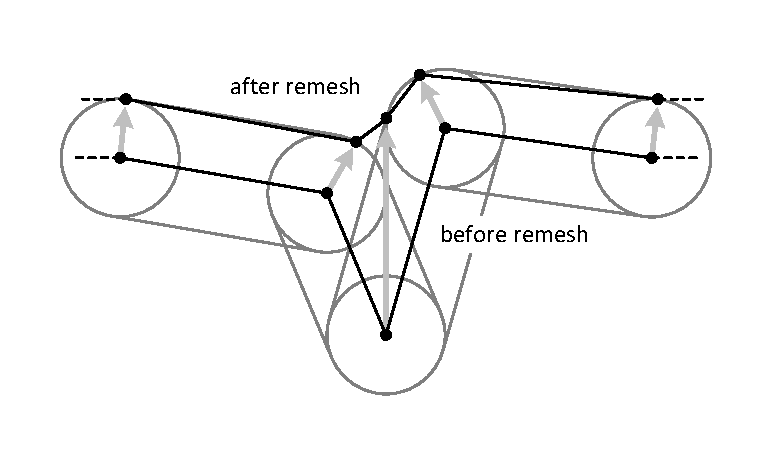
\includegraphics[width=\textwidth]{pics/pic_general_envelope_3_size.pdf}
    \caption{Иллюстрация затягивания впадины на 2D схеме.}\label{fig:pic_general_envelope_3_size}
  \end{minipage}
  \hfill
  \begin{minipage}[h]{0.44\textwidth}
    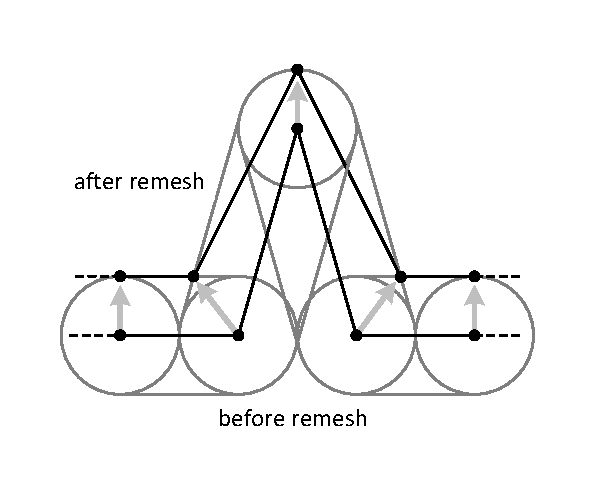
\includegraphics[width=\textwidth]{pics/pic_general_envelope_4_size.pdf}
    \caption{Иллюстрация сглаживания острого пика на 2D схеме.}\label{fig:pic_general_envelope_4_size}
  \end{minipage}
\end{figure}

\begin{figure}[h]
  \centering
  \begin{minipage}[h]{0.49\textwidth}
    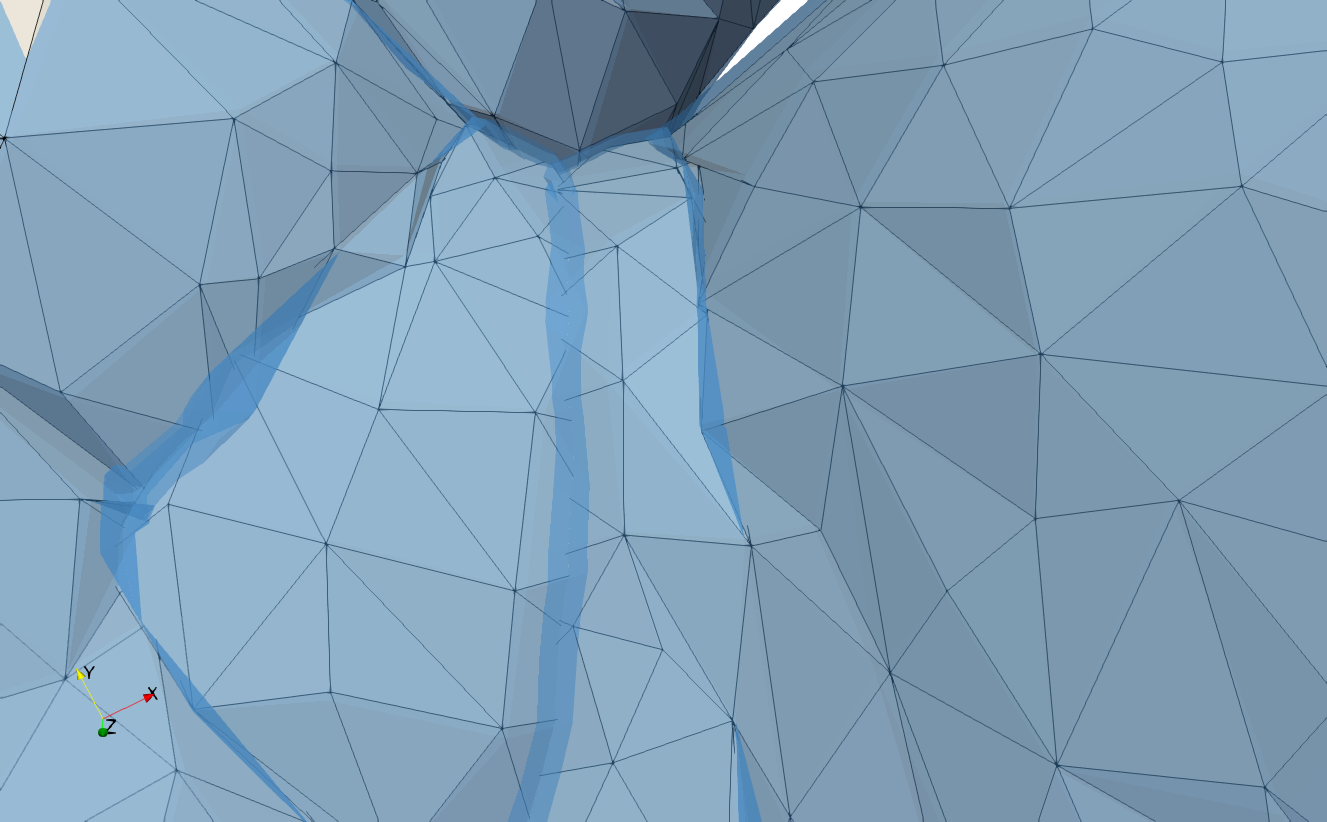
\includegraphics[width=\textwidth]{pics/pic_envelope_cave.png}
    \caption{Иллюстрация затягивания впадин для 3D поверхности.}\label{fig:pic_general_envelope_cave}
  \end{minipage}
  \hfill
  \begin{minipage}[h]{0.49\textwidth}
    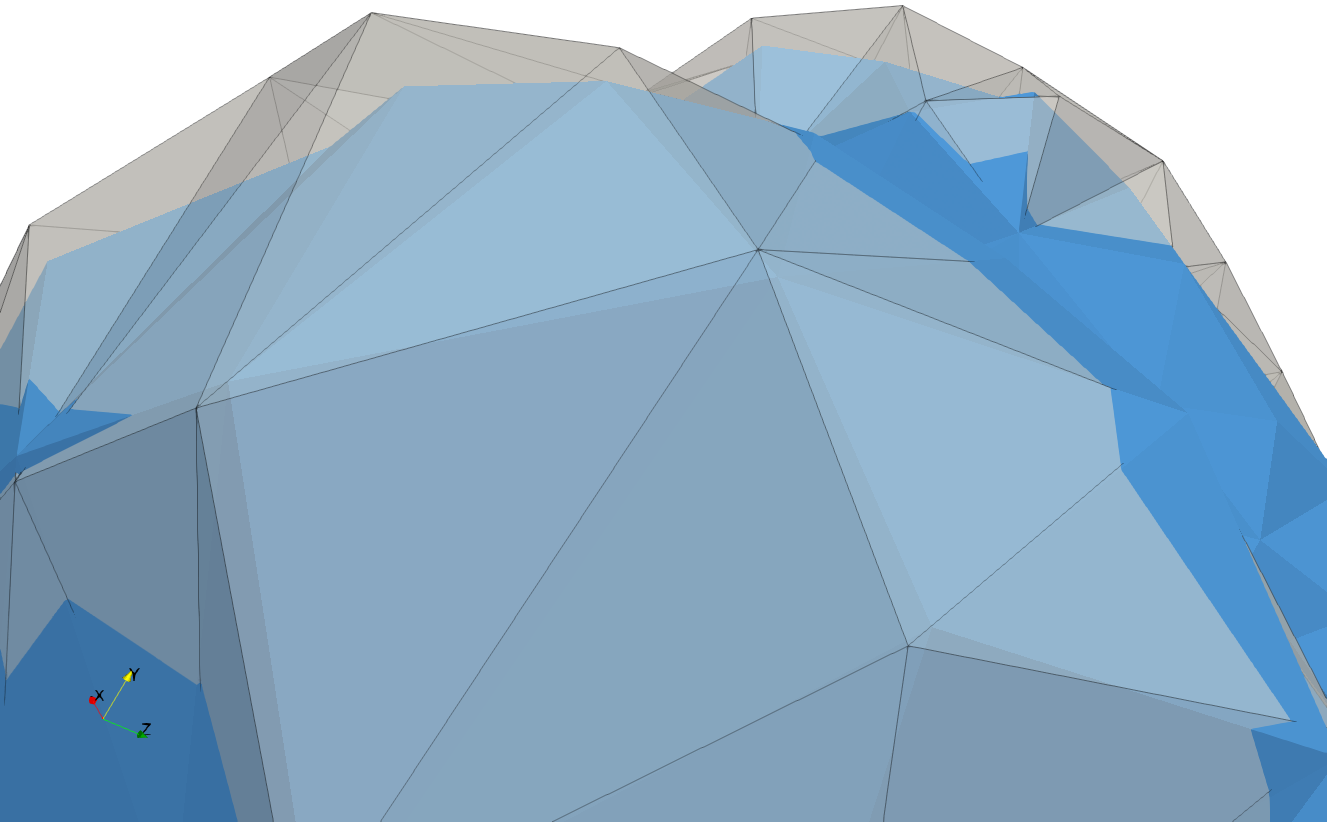
\includegraphics[width=\textwidth]{pics/pic_envelope_peak.png}
    \caption{Иллюстрация сглаживания острых пиков для 3D поверхности.}\label{fig:pic_envelope_peak}
  \end{minipage}
\end{figure}

Алгоритм определения новых положений узлов по общей огибающей семейства сфер является линейным по количеству узлов (считаем, что на пригодных к расчетам сетках количество инцидентных ячеек для одного узла ограничено разумным числом) и не содержит итерационных процедур.
Алгоритм обладает особенностью затягивать мелкие впадины и шумы на сетке.
Это происходит из-за того, что узел $\vec{N}$, находясь на дне впадины, имеет возможность смещаться по направлению выхода из этой впадины на расстояние, большее $R(\vec{N})$, что продемонстрировано на Fig.~\ref{fig:pic_general_envelope_3_size}.
Другой интересной особенностью является работа алгоритма на участках сетки с острыми выступами (Fig.~\ref{fig:pic_general_envelope_4_size}).
Из данного рисунка видно, что в процессе работы алгоритма острые пики имеют тенденцию к сглаживанию. 
Таким образом, новые положения узлов образуют более гладкую поверхность, чем она была до перестроения.

На Fig.~\ref{fig:pic_general_envelope_cave} продемонстрирован эффект затягивания впадин по сравнению с классическим методом призм (затягивание впадин на сетке отмечено синим цветом). На Fig.~\ref{fig:pic_envelope_peak} показан обратный эффект -- сглаживание острых пиков (по сравнению с тем же классическим методом призм).

%---------------------------------------------------------------------------------------------------

\section{Adaptation}

Все рассмотренные в предыдущем разделе методы перестроения поверхностей объединяет одно сходство -- они сохраняют количество элементов расчетной сетки (узлы, ребра, грани) и связи между ними.
Несмотря на некоторые специальные методы по предотвращению конфликтов между гранями сетки и методы сглаживания, после формирования новой поверхности возможно возникновение самопересечений, появление граней неправильной формы, а также неравномерное распределение граней в сетке по размеру.
Пока опустим самопересечения сетки и будем рассматривать только вопросы, касающиеся формы и размера ячеек.

\begin{figure}[h]
  \centering
  \begin{minipage}[h]{0.35\textwidth}
    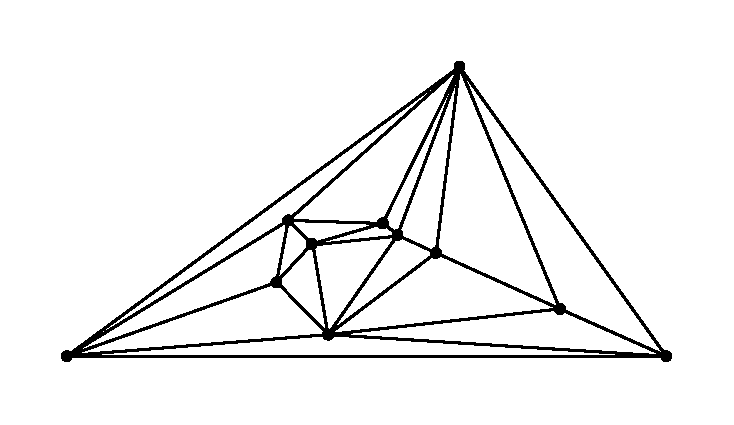
\includegraphics[width=\textwidth]{pics/pic_delaunay_size.pdf}
    \caption{Разбиение ячейки с помощью триангуляции Делоне.}\label{fig:pic_delaunay}
  \end{minipage}
  \hfill
  \begin{minipage}[h]{0.35\textwidth}
    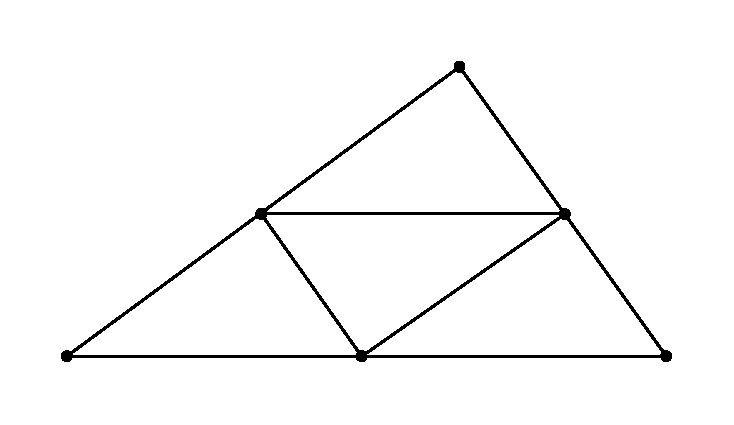
\includegraphics[width=\textwidth]{pics/pic_delaunay_2_size.pdf}
    \caption{Дробление ячейки на более мелкие.}\label{fig:pic_delaunay_2}
  \end{minipage}
  \hfill
  \begin{minipage}[h]{0.28\textwidth}
    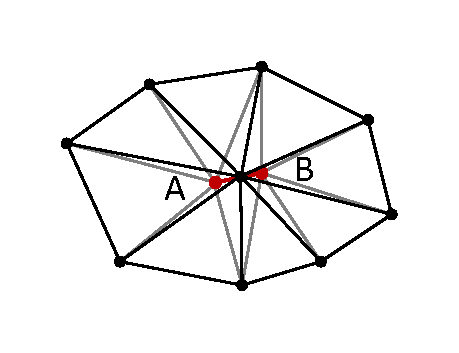
\includegraphics[width=\textwidth]{pics/pic_reduce_edge_size.pdf}
    \caption{Стягивание ребра.}\label{fig:pic_reduce_edge}
  \end{minipage}
\end{figure}

Первая операция, которая нам потребуется -- разбиение ячейки на более мелкие.
Во всех случаях будем выполнять разбиение ячеек с помощью триангуляции Делоне, считая что для разбиения нам известен набор точек внутри разбиваемой ячейки (Fig.~\ref{fig:pic_delaunay}) \cite{Rivara}.
Стоит отметить, что разбиение ячейки можно производить с сохранением локальной кривизны сетки, как это показано в \cite{Rakotoarivelo}, но для простоты будем производить разбиение исключительно в плоскости ячейки.
Если точка разбиения находится не внутри ячейки, а на ее ребре, то разбить придется также вторую инцидентную ячейку этого ребра (рассматриваются только сетки, ребра которых имеют ровно по две инцидентные ячейки, как это указано в (\ref{eq_arch}).
Иногда для уменьшения размера требуется просто разбить ячейку на более мелкие без задания точек разбиения.
В этом случае необходимо следить за качеством результирующих ячеек.
Для определения качества формы ячейки треугольной формы с узлами $\vec{A}$, $\vec{B}$, $\vec{C}$ можно пользоваться простым критерием качества

\begin{equation}
Q(f) = \frac{4\sqrt{3} S_{ABC}}{|\vec{AB}|^2 + |\vec{BC}|^2 + |\vec{AC}|^2}
\end{equation}

где $Q(f) = 1$ соответствует идеальному случаю равносторонней ячейки, а $Q(f) = 0$ -- худший случай для ячеек с нулевой площадью \cite{Borouchaki}.
Для выполнения разбиения ячейки на более мелкие с сохранением их качества просто выполним разбиение по серединам всех ее сторон (Fig.~\ref{fig:pic_delaunay_2}).

Вторая операция, которая необходима для адаптации сетки, связана с огрублением.
Достаточно часто во время выполнения триангуляции по множеству заданных точек могут появляться ячейки с низким показателем качества (у них могут присутствовать либо слишком острые углы, либо близкий к развернутому угол).
Если в ячейке присутствует угол, близкий к развернутому, то избавиться от него поможет разбиение по наибольшей стороне (при этом в качестве точки разбиения следует выбрать основание высоты, опущенной из противолежащего узла).
Если же в треугольнике присутствуют лишь близкие к острым углы, то значит в нем есть слишком короткая сторона, которая может быть удалена.
При удалении ребра $AB$ удаляются обе инцидентные ей грани, узлы $A$ и $B$ соединяются в единый узел $A'$, а все ребра из множества $\mathscr{E}(A) \cup \mathscr{E}(B)$ перенаправляются на узел $A'$ с учетом удаления повторных (Fig.~\ref{fig:pic_reduce_edge}).
Данную операцию будем называть стягиванием ребра \cite{Panchal}.
Путем применения стягивания наиболее коротких ребер в расчетной сетке можно добиться произвольной степени огрубления.

%---------------------------------------------------------------------------------------------------

\section{Устранение самопересечений}

Основной проблемой, с которой можно потенциально столкнуться при эволюции расчетной сетки, является возникновение самопересечений.
Самопересечение является критическим дефектом сетки, при котором невозможно производить дальнейшие вычисления по моделированию ледообразования, поэтому самопересечения необходимо удалять.
Во-первых, необходимо определить, какое отношение двух ячеек сетки можно трактовать как самопересечение.
Конечно, простое наличие общих точек у двух ячеек не может служить критерием самопересечения, так как у каждой ячейки есть смежные ячейки (то есть две ячейки могут иметь как общую вершину, так и общее ребро).
Так как смежными могут быть только ячейки, имеющие общие инцидентные объекты (общую инцидентную вершину или общее инцидентное ребро), а все отношения инцидентности прописаны в расчетной сетке, то не представляет труда отделить пересечение ячеек по общему инцидентному объекту от самопересечения.

\subsection{Поиск пар пересекающихся треугольников}

В любом случае для идентификации всех фактов самопересечения сетки требуется проанализировать все пары ячеек и проверить пересечение ячеек в паре (то есть проверить пересечение каждой ячейки с каждой).
Так как прямой перебор всех пар ячеек имеет квадратичную сложность по количеству ячеек в сетке, то его использование на крупных сетках невозможно.
В этом случае целесообразно выполнять поиск пар пересекающихся ячеек с помощью представления множества ячеек в виде специальной древовидной структуры, связанной с ограничением геометрических объектов прямоугольными параллелепипедами в пространстве.
Для начала определим понятие контейнера для произвольного множества точек $M$ в пространстве (будем обозначать его через $[M]$): $[M]$ -- это прямоугольный параллелепипед, являющийся декартовым произведением трех сегментов

\begin{equation}
[M] = \left[\min_{P \in M}{P_x}, \max_{P \in M}{P_x}\right]
      \times \left[\min_{P \in M}{P_y}, \max_{P \in M}{P_y}\right]
      \times \left[\min_{P \in M}{P_z}, \max_{P \in M}{P_z}\right]
\end{equation}

Контейнер можно рассматривать для произвольного множества точек.
Мы будем его использовать для ячейки расчетной сетки, а также для множества ячеек.
Так как любой треугольник является выпуклой фигурой, то $[ABC] = [\{A, B, C\}]$, то есть для построения контейнера для треугольника достаточно рассмотреть только его вершины.
При поиске пар пересекающихся ячеек будем использовать следующий факт: если два треугольника пересекаются, то пересекаются и их контейнеры: $ABC \cap A'B'C' \ne \emptyset \Rightarrow [ABC] \cap [A'B'C'] \ne \emptyset$.
А значит если не пересекаются контейнеры двух треугольников, то не пересекаются и сами треугольники: $[ABC] \cap [A'B'C'] = \emptyset \Rightarrow ABC \cap A'B'C' = \emptyset$.
В отличие от анализа пары треугольников на пересечение, проверка на пересечение двух прямоугольных параллелепипедов со сторонами, параллельными координатным осям, не представляет проблем.
То есть па первом этапе будем искать такие пары ячеек, чьи контейнеры пересекаются (будем называть их потенциально пересекающимися ячейками).

\begin{figure}[h]
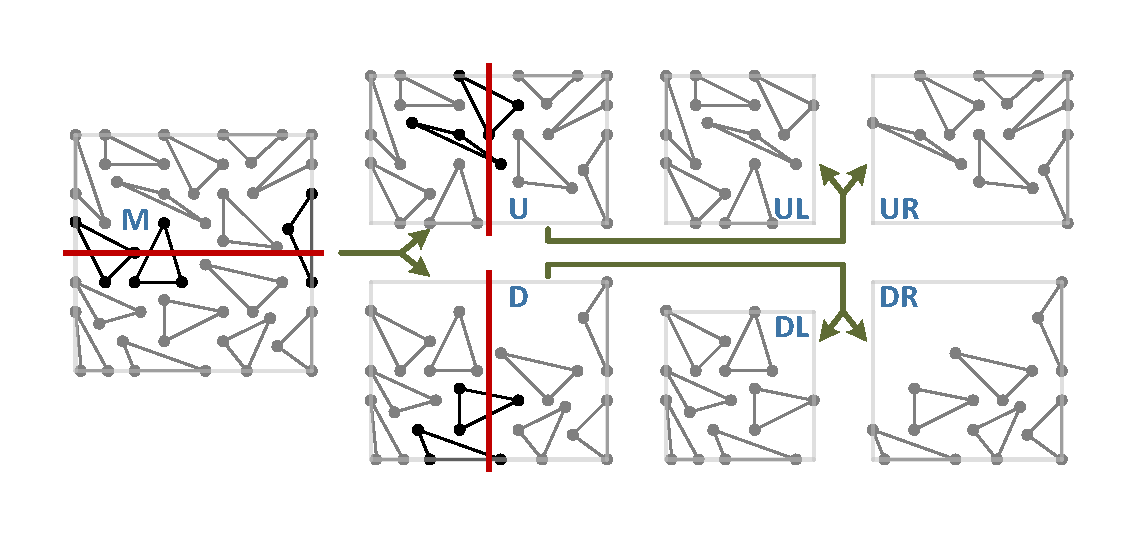
\includegraphics[width=0.8\textwidth]{pics/pic_box_size.pdf}
\captionstyle{center}\caption{Схема построения дерева контейнеров.}\label{fig:pic_box}
\end{figure}

Для поиска потенциально пересекающихся ячеек построим дерево контейнеров всех ячеек сетки.
Корнем данного дерева будет являться контейнер всех ячеек расчетной сетки.
Рассмотрим процедуру разделения контейнера на два более мелких на примере двумерного случая, проиллюстрированного на Fig.~\ref{fig:pic_box}.
Путь мы хотим разделить контейнер некоторого множества треугольников ($M$) по горизонтальной прямой на два множества: верхнее ($U$) и нижнее ($D$).
Тогда в верхнее множество попадут все треугольники, лежащие выше прямой, либо пересекающие ее.
Аналогично в нижнее множество попадут все треугольники, лежащие ниже прямой, либо пересекающие ее.
После выделения верхнего и нижнего множества треугольников, для каждого из них строятся свои контейнеры, которые становятся дочерними контейнерами исходного.
После этого получившиеся контейнеры можно делить дальше, используя произвольное направление разбиения ($X$, $Y$, $Z$).
В частности на Fig.~\ref{fig:pic_box} продемонстрировано разбиение исходного контейнера по схеме $[M] \rightarrow \{[U], [D]\} \rightarrow \{\{[UL], [UR]\}, \{[DL], [DR]\}\}$.
Следует заметить, что за одну операцию контейнер можно разбивать на произвольное количество дочерних контейнеров аналогичным образом.
В качестве же направления разбиения контейнера целесообразно выбирать наиболее протяженное (вдоль которого длина контейнера имеет наибольшее значение).

Построенное дерево контейнеров позволяет существенно сократить количество проверяемых потенциальных пересечений треугольников \cite{Jung}, так как если $[M] \cap [M'] = \emptyset$, $[T]$ -- дочерний контейнер для $[M]$, а $[T']$ -- дочерний контейнер для $[M']$, то $[T] \cap [T'] = \emptyset$.

После того, как найдены все пары потенциально пересекающихся треугольников, необходимо проверить, пересекаются ли они на самом деле.
Так как треугольник является выпуклой фигурой, то пересечение двух треугольников также является выпуклой фигурой (это может быть любая плоская фигура с количеством вершин от 1 до 6).
Вершинами пересечения двух треугольников являются точки пересечения сторон одного треугольника с другим треугольником и наоборот.
Таким образом задача поиска пересечения двух треугольников сводится к поиску точек пересечения треугольника и отрезка.
Данная задача может быть решена, с помощью представления треугольника $ABC$ в виде геометрического места точек $\vec{P} = \vec{A} + \beta \vec{AB} + \gamma \vec{AC}$, $\beta \ge 0$, $\gamma \ge 0$, $\beta + \gamma \le 1$, представления отрезка $QR$ в виде геометрического места точек $\vec{P} = \vec{Q} + \phi \vec{QR}$, $0 \le \phi \le 1$ и поиска решения системы уравнений $\vec{A} + \beta \vec{AB} + \gamma \vec{AC} = \vec{Q} + \phi \vec{QR}$ относительно неизвестных $\beta$, $\gamma$, $\phi$ с учетом ограничений \cite{Freylekhman}.

\subsection{Фиксация пересекающихся треугольников}

После того, как найдены все пары пересекающихся ячеек и области их пересечения, необходимо определить стратегию их устранения.
Все ячейки расчетной сетки можно разделить на три категории.
Первая категория -- ячейки, которые не пересекаются ни с какими другими ячейками, и которые должны стать частью итоговой поверхности (будем считать, что в любой момент времени у нас есть возможность указать произвольное количество таких ячеек).
Будем такие ячейки называть статические.
Вторая категория -- ячейки, которые не пересекаются ни с какими другими ячейками, но которые не должны стать частью итоговой поверхности (ячейки внутренних петель самопересечения поверхности, которые должны быть удалены).
Такие ячейки будем называть скрытыми.
Третья категория -- ячейки, которые пересекаются с какими-то другими ячейками. 
Такие ячейки будем называть ячейками пересечения.

\begin{figure}[h]
  \centering
  \begin{minipage}[h]{0.32\textwidth}
    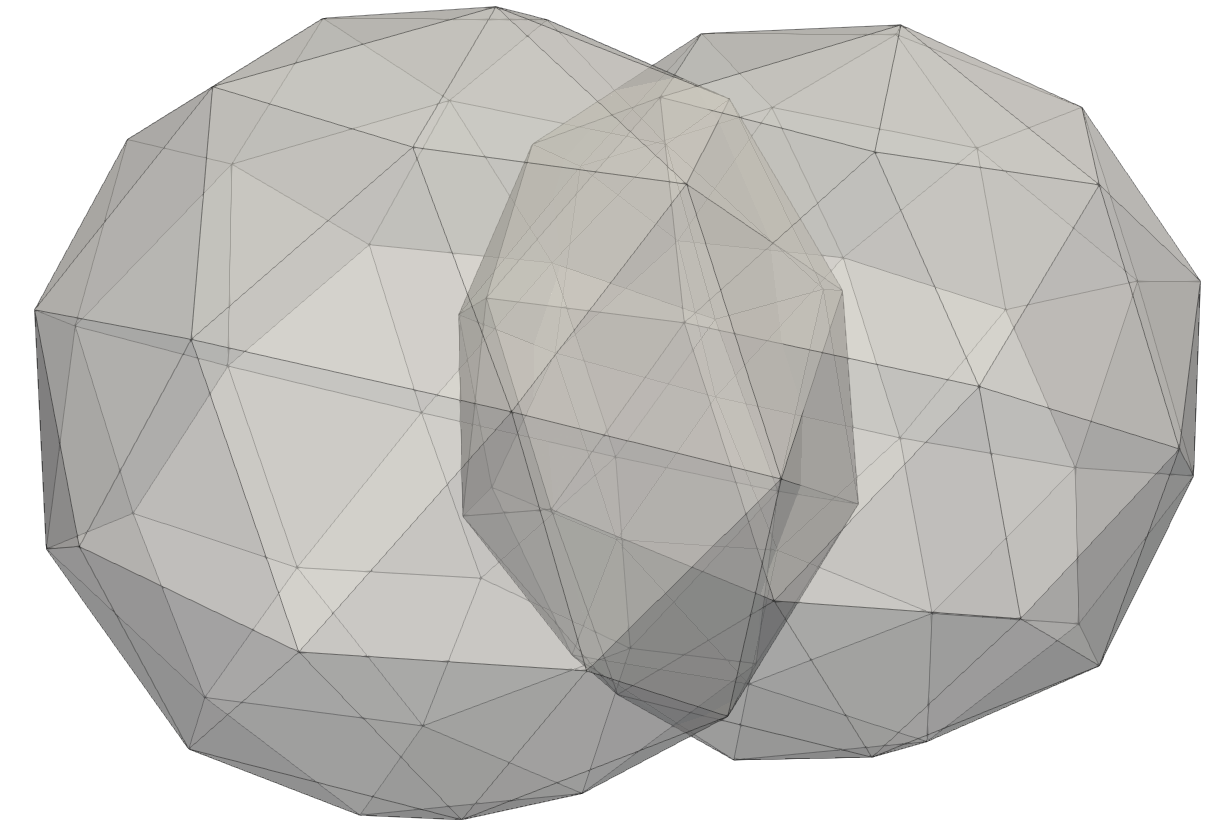
\includegraphics[width=\textwidth]{pics/pic_zip_01.png}
    \caption{Пересечение расчетных сеток для двух сфер.}\label{fig:pic_zip_01}
  \end{minipage}
  \hfill
  \begin{minipage}[h]{0.32\textwidth}
    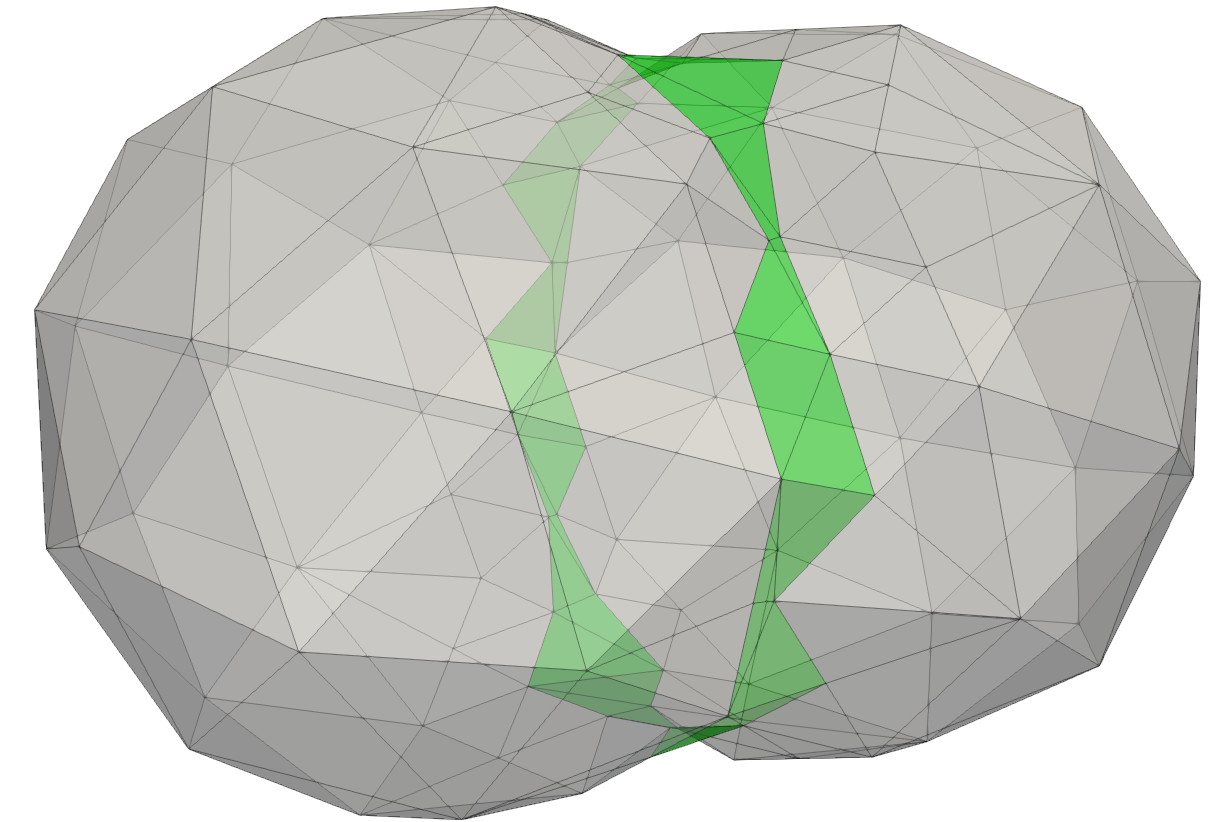
\includegraphics[width=\textwidth]{pics/pic_zip_09.png}
    \caption{Грубое удаление ячеек пересечения.}\label{fig:pic_zip_09}
  \end{minipage}
  \hfill
  \begin{minipage}[h]{0.32\textwidth}
    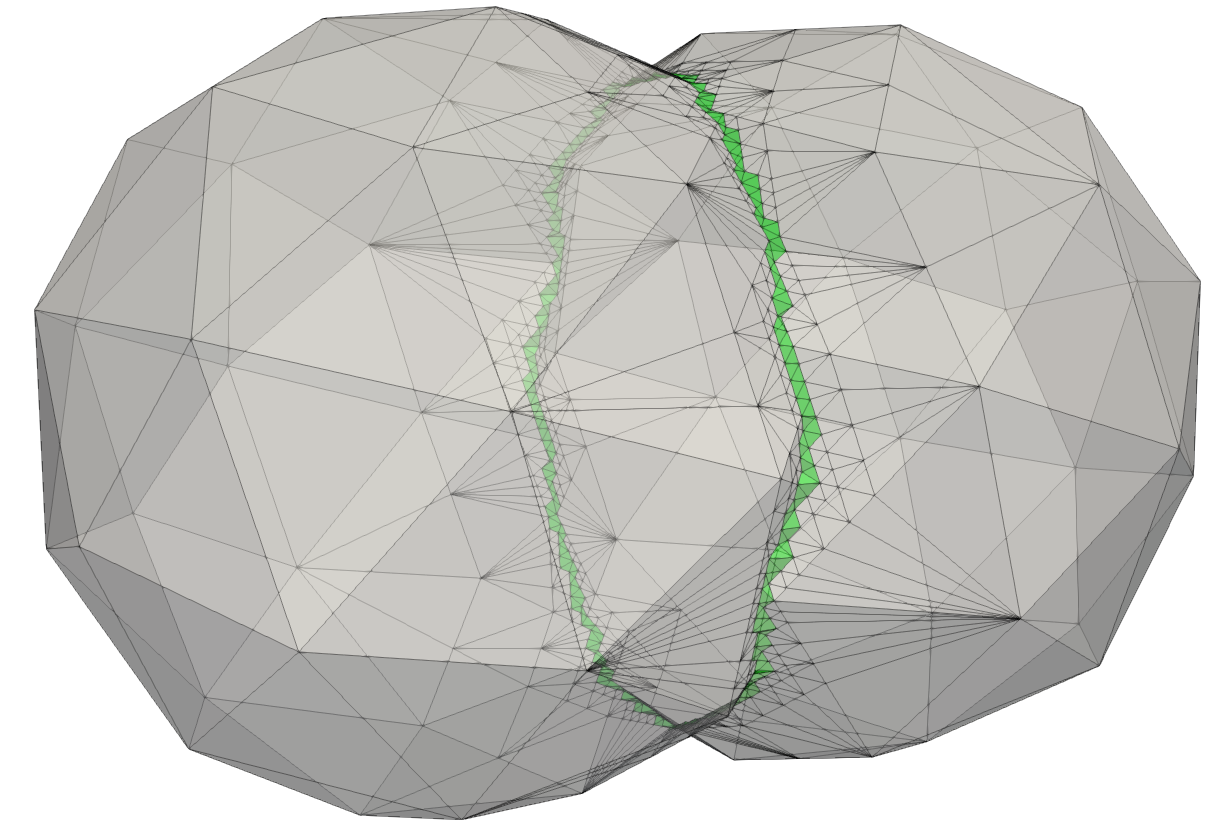
\includegraphics[width=\textwidth]{pics/pic_zip_15.png}
    \caption{Удаление ячеек пересечения после дробления.}\label{fig:pic_zip_15}
  \end{minipage}
\end{figure}

Одним из подходов к устранению самопересечений сетки является просто удаление всех ячеек пересечения.
После выполнения этой операции сетка распадается на области статических и скрытых ячеек.
При этом скрытые ячейки являются недостижимыми из статических при выполнении обхода ячеек расчетной сетки (если в процессе обхода соседними считаются только ячейки, смежные по ребру).
После удаления из сетки скрытых ячеек расчетная сетка состоит только из статических ячеек, однако требуется добавление новых ячеек для восстановления целостности сетки \cite{Charton}.
Такой подход к устранению самопересечений сетки может применяться для сравнительно простых поверхностей, но в общем случае он не гарантирует получение корректного результата.
В качестве иллюстрации такого способа устранения пересечений на Fig.~\ref{fig:pic_zip_01}, Fig.~\ref{fig:pic_zip_09} приведен пример работы для устранения пересечений расчетных сеток двух сфер (новые ячейки, появляющиеся при восстановлении сетки отмечены зеленым цветом).
На Fig.~\ref{fig:pic_zip_09} можно отметить, достаточно низкое качество результирующей сетки.
Повысить качество можно с помощью дробления ячеек пересечения.
То есть после поиска всех ячеек пересечения, их необходимо раздробить на более мелкие (как показано на Fig.~\ref{fig:pic_delaunay_2}), после чего повторить процедуру удаления ячеек пересечения и скрытых ячеек и выполнить восстановление сетки.
Процесс дробления ячеек пересечения можно повторять многократно, при этом качество результирующей сетки будет повышаться, как это показано на Fig.~\ref{fig:pic_zip_15}.

При другом подходе устранения самопересечений никакие ячейки из сетки не удаляются, а дробятся на более мелкие по всем точкам пересечения \cite{Skvorkovska}.
В качестве примера на Fig.~\ref{fig:pic_before_cut} показаны два треугольника, которые пересекаются по отрезку (две точки пересечения).
После выполнения дробления получаем конструкцию, показанную на Fig.~\ref{fig:pic_after_cut}.
В общем случае точек, по которым необходимо разбивать ячейку, может быть сколь угодно много, и дробление должно выполняться с помощью выполнения триангуляции по этим точкам, причем некоторые ребра триангуляции должны быть фиксированы.

\begin{figure}[h]
  \centering
  \begin{minipage}[h]{0.4\textwidth}
    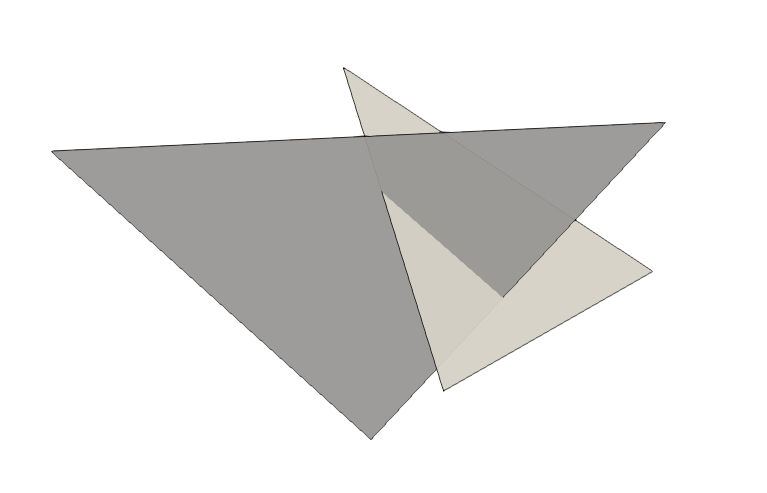
\includegraphics[width=\textwidth]{pics/pic_before_cut.png}
    \caption{Два пересекающихся треугольника до дробления.}\label{fig:pic_before_cut}
  \end{minipage}
  \begin{minipage}[h]{0.4\textwidth}
    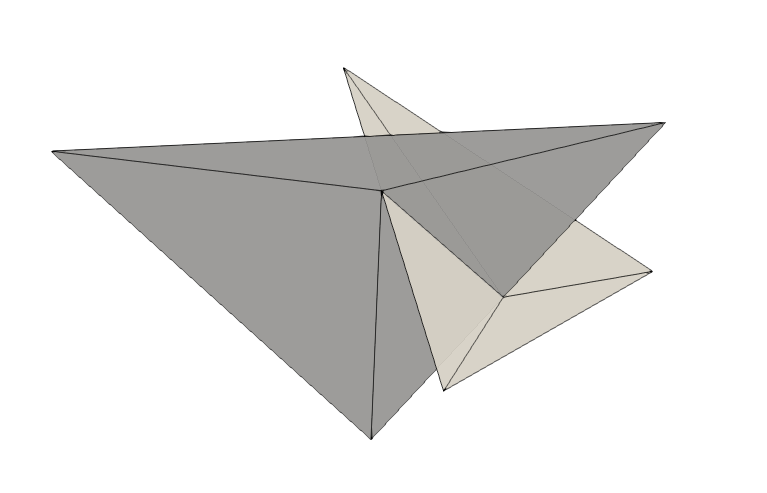
\includegraphics[width=\textwidth]{pics/pic_after_cut.png}
    \caption{Ячейки после дробления по точкам пересечения.}\label{fig:pic_after_cut}
  \end{minipage}
\end{figure}

После дробления ячеек по точкам пересечения, между ячейками сетки могут остаться только следующие виды отношений: две ячейки не имеют общих точек, две ячейки имеют одну общую вершину, две ячейки имеют одно общее ребро.
При этом в сетке появляются ребра, имеющие более двух инцидентных ячеек.
Если наложить на исходную сетку два дополнительных условия, которые могут быть достигнуты с помощью локальных преобразований сетки, то можно добиться достаточно простой структуры сетки (такие сетки будем называть простыми).
Первым условием будем считать отсутствие в сетке совпадающих вершин.
Вторым условием будем считать то, что никакой узел сетки не находится ни в какой другой ячейке.
При выполнении этих двух дополнительных условий можно утверждать, что если ребро имеет более двух инцидентных ячеек, то это количество в точности равно 4, причем эти 4 инцидетные ячейки попарно находятся в одной плоскости.

\begin{figure}[h]
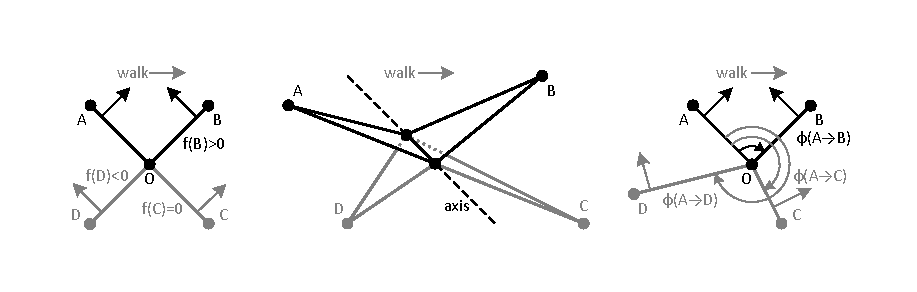
\includegraphics[width=1.0\textwidth]{pics/pic_walk_1_size.pdf}
\captionstyle{center}\caption{Схема обхода результирующей поверхности.}\label{fig:pic_walk}
\end{figure}

Для получения результирующей поверхности необходимо избавиться от лишних ячеек, чтобы у каждого ребра вновь осталось ровно по 2 инцидентные ячейки.
Для этого нужно выполнить обход сетки, начиная с любой статической ячейки, считая соседними две ячейки, имеющие общее инцидентное ребро (помечаемые в процессе обхода ячейки попадут в результирующую сетку).
При движении от некоторой ячейки через ребро, имеющее более двух инцидентных ячеек, возникает вопрос выбора ячейки, которая должна войти в результирующую сетку (при этом все остальные ячейки должны быть удалены).

Рассмотрим процедуру выбора следующей ячейки обхода сетки для ребер, имеющих количество инцидентных ячеек, больше двух (Fig.~\ref{fig:pic_walk}, в центре).
На данном рисунке обозначено направление обхода слева направо, вслед за ячейкой, инцидентной вершине $A$, в результирующую сетку должна войти ячейка, инцидентная вершине $B$.
Рассмотрим эту процедуру для простых сеток, а также для сеток в общем виде.
Для простоты будем рассматривать задачу в проекции на плоскость, перпендикулярную ребру.

Для начала будем считать, что имеет место случай простой сетки (Fig.~\ref{fig:pic_walk}, слева).
Пусть уже известно, что ячейка, инцидентная вершине $A$, помечена, а ее внешняя нормаль равна $\vec{n}_A$.
Из оставшихся трех ячеек (инцидентных вершинам $B$, $C$, $D$ соответственно) необходимо выбрать только одну для продолжения обхода сетки, а остальные удалить.
Так как сетка у нас простая, то $\angle AOC = \angle BOD = 2 \pi$, а значит $(\vec{n}_A, \vec{OB}) > 0$, $(\vec{n}_A, \vec{OC}) = 0$, $(\vec{n}_A, \vec{OD}) < 0$.
Таким образом, из всех ячеек, необходимо выбрать ту, для которой значение $(\vec{n}_A, \vec{OP})$ максимально.

Теперь рассмотрим расчетную сетку в общем виде.
В этом случае количество ячеек, инцидентных рассматриваемому ребру, может быть произвольным, больше двух, а про значение функции $(\vec{n}_A, \vec{OP})$ сказать ничего нельзя.
Для выбора следующей ячейки для обхода сетки будем поворачивать текущую ячейку вокруг рассматриваемого ребра в направлении $\vec{n}_A$ до совпадения с первой ячейкой (Fig.~\ref{fig:pic_walk}, справа).
Первая ячейка и должна быть выбрана в качестве следующей для продолжения обхода.
Если через $\phi(A \rightarrow P)$  обозначить угол поворота исходной ячейки в направлении $\vec{n}_A$ до ячеки, инцидентной вершине $P$, то в качестве следующей ячейки для обхода необходимо выбрать ту, для которой $\phi(A \rightarrow B)$ будет минимально.

\begin{figure}[h]
  \centering
  \begin{minipage}[h]{0.49\textwidth}
    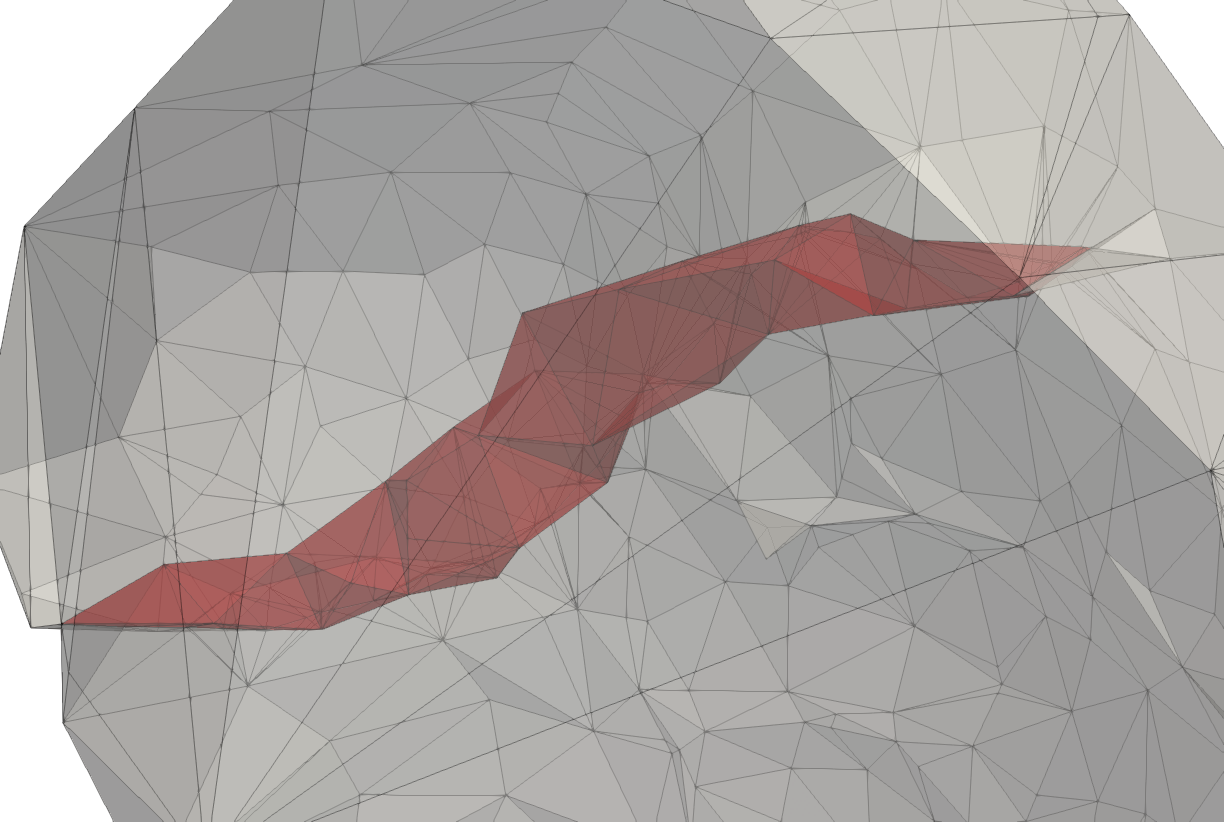
\includegraphics[width=\textwidth]{pics/pic_self_intersection_on.png}
    \caption{Поверхность до удаления самопересечения.}\label{fig:pic_self_intersection_on}
  \end{minipage}
  \hfill
  \begin{minipage}[h]{0.49\textwidth}
    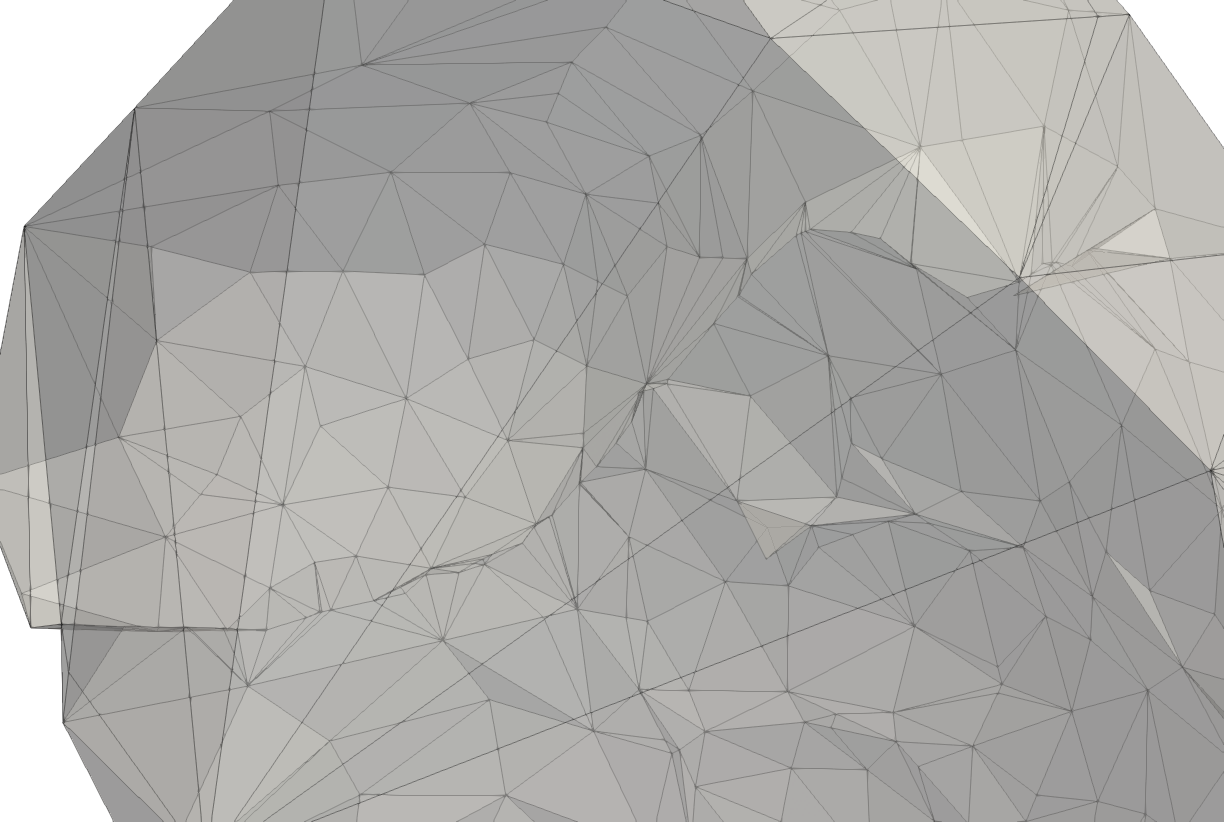
\includegraphics[width=\textwidth]{pics/pic_self_intersection_off.png}
    \caption{Поверхность после удаления самопересечения.}\label{fig:pic_self_intersection_off}
  \end{minipage}
\end{figure}

\begin{figure}[h]
  \centering
  \begin{minipage}[h]{0.49\textwidth}
    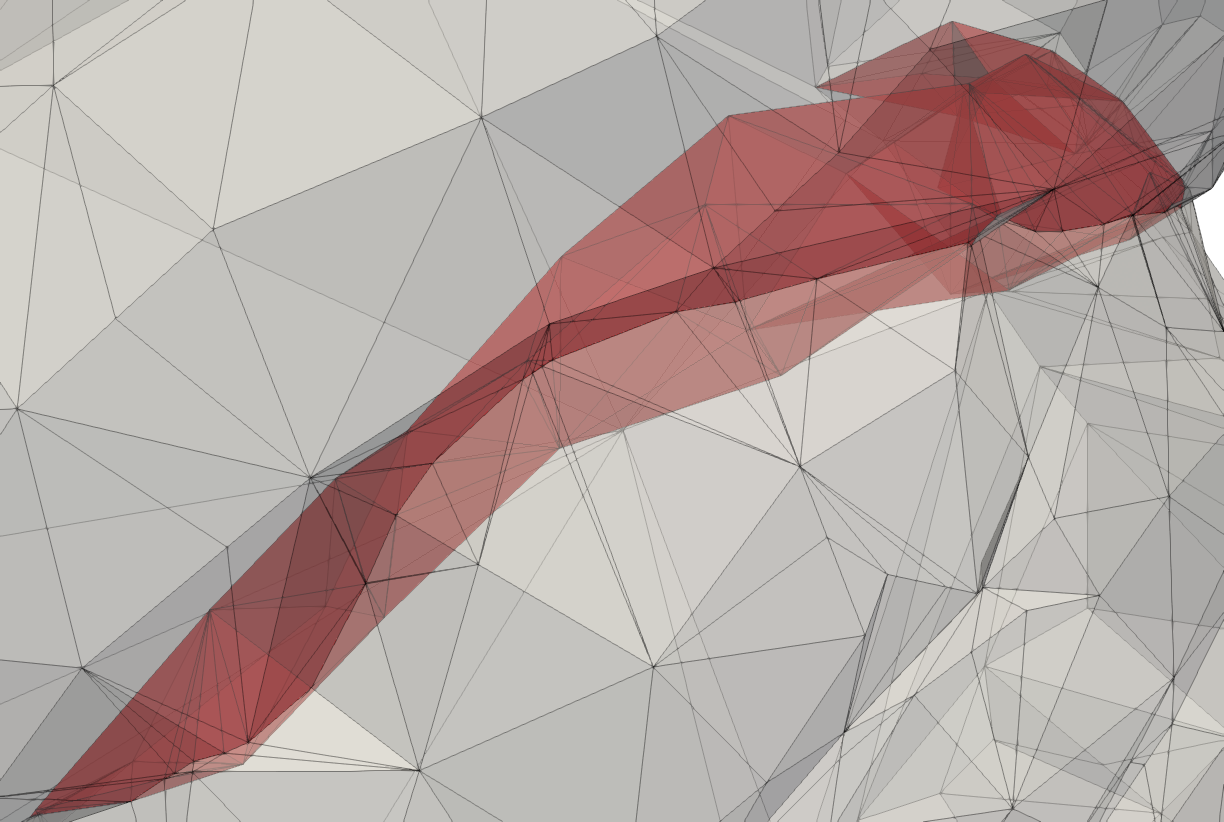
\includegraphics[width=\textwidth]{pics/pic_self_intersection_on_2.png}
    \caption{Поверхность до удаления самопересечения.}\label{fig:pic_self_intersection_on_2}
  \end{minipage}
  \hfill
  \begin{minipage}[h]{0.49\textwidth}
    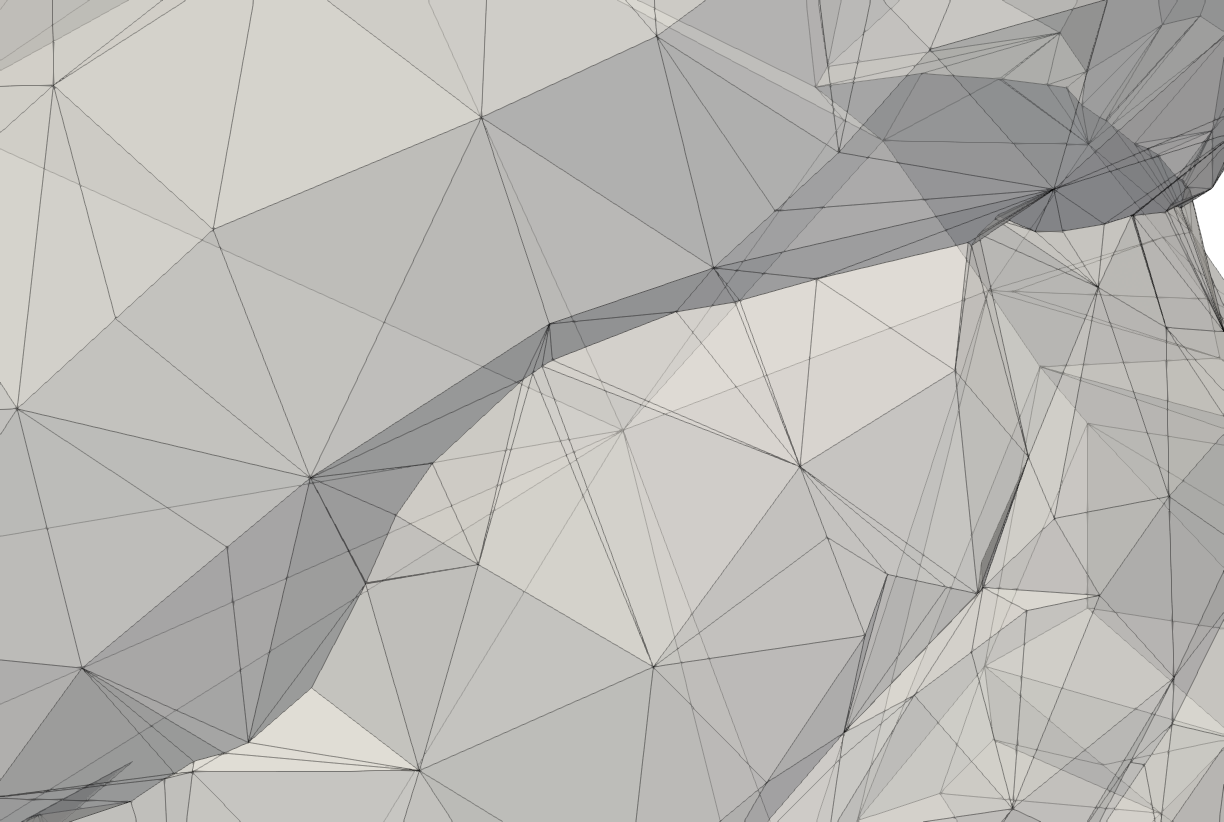
\includegraphics[width=\textwidth]{pics/pic_self_intersection_off_2.png}
    \caption{Поверхность после удаления самопересечения.}\label{fig:pic_self_intersection_off_2}
  \end{minipage}
\end{figure}

Объединяя вместе оба рассмотренных случая, получаем критерий выбора следующей для обхода ячейки: должна быть выбрана ячейка, для которой значение показателя $f(P)$ максимально, где

\begin{equation}
f(P) = 
\begin{cases}
(\vec{n}_A, \vec{OP}), \text{для простых сеток}, \\
-\phi(A \rightarrow P), \text{для сеток общего вида}
\end{cases}
\end{equation}

После завершения обхода расчетной сетки все помеченные ячейки считаются ячейками целевой поверхности, а все остальные ячейки должны быть удалены.
На рисунках Fig.~\ref{fig:pic_self_intersection_on} -- Fig.~\ref{fig:pic_self_intersection_off_2} проиллюстрированы примеры устранения самопересечений сетки в виде скрытых петель.
После удаления скрытых ячеек целевая расчетная сетка снова становится корректной, удовлетворяет соотношениям (\ref{eq_arch}) и может быть использована для дальнейшего моделирования ледообразования.

%---------------------------------------------------------------------------------------------------

\section{Conclusion}

В статье рассмотрен геометрический аспект задачи моделирования процесса ледообразования, а именно задача эволюции неструктурированной поверхностной расчетной сетки.
В процессе эволюции изменение положения узлов сетки должно соответствовать объему накопленного льда в ячейках сетки, а сама сетка должна оставаться корректной, целостной и не содержать самопересечений.
В противном случае продолжение моделирования процесса ледообразования может оказаться невозможным.

Эволюция расчетной сетки состоит из двух основных этапов.
На первом этапе происходит вычисление новых положений узлов сетки в соответствии с объемом накопленного льда.
Был рассмотрен ряд наиболее распространенных алгоритмов вычисления новых положений узлов, а также предложен новый алгоритм.
Среди рассмотренных алгоритмов вычисления новых положений узлов присутствовали классические алгоритмы явного вычисления координат узлов, базирующиеся на аппроксимации объема льда в виде простых геометрических фигур (метод призм и метод пирамид).
Был рассмотрен многослойный подход, моделирующий итерационное наращивания льда отдельными слоями, позволяющий существенно повысить точность классических методов.
Был рассмотрен алгоритм перестроения поверхности, использующий перемещение вершин с сохранением объема, основными особенностями которого являются пошаговое перестроение, вычисление максимальной доли наращиваемого льда для предотвращения локального самопересечения и применение сглаживаний различного вида для эффективной обработки впадин на поверхности тела.
Был предложен новый алгоритм перестроения поверхности, основанный на формировании новой поверхности в виде общей огибающей семейства сфер, центры которых расположены на исходной поверхности, а радиусы соответствует интенсивности нарастания льда.
Предложенный алгоритм является линейным по количеству ячеек сетки, устойчивым, а также имеет тенденцию к затягиванию небольших трещин и впадин на поверхности и к сглаживанию острых пиков и изломов.

Так как вне зависимости от применяемого алгоритма перестроения поверхности невозможно дать гарантию отсутствия самопересечения результирующей сетки, то в качестве второго этапа эволюции сетки рассматривалось удаление этих самопересечений.
Было рассмотрено два подхода к устранению самопересечений.
В основе обоих подходов лежит поиск пересечений ячеек сетки с другими ячейками, отличными от смежных (ячеек пересечения).
В основе первого подхода устранения самопересечений является удаление ячеек пересечения с последующим восстановлением сетки.
В качестве второго подхода рассматривался метод, основанный на дроблении всех ячеек сетки по точкам пересечения с другими ячейками, обходе расчетной сетки начиная со статической области и удаления после данного обхода всех непомеченных ячеек.

Все рассмотренные методы перестроения поверхностей и устранения самопересечений были реализованы и протестированы на предмет применимости в задачах моделирования ледообразования.
По итогам проведенного тестирования в качестве практического использования был выбран механизм перестроения поверхности, основанный на общей огибающей семейства сфер (так как данный алгоритм является быстрым, надежным и помогает снижать дефекты сетки).
В качестве алгоритма устранения самопересечений сетки предпочтение было отдано алгоритму, основанному на дроблении ячеек по точках пересечения.
Данный алгоритм, хоть и является достаточно медленным (за счет необходимости анализа на пересечение всех потенциально конфликтующих пар ячеек), однако применим к расчетным сеткам произвольной геометрии и сложности.

\begin{acknowledgments}
The work was carried out at the JSCC RAS as part of the government assignment (topic FNEF-2022-0016). Supercomputer MVS-10P was used in research.
\end{acknowledgments}

%---------------------------------------------------------------------------------------------------

\begin{thebibliography}{99}

% Introduction.

\bibitem{Raj}
\refitem{article}
L.~Prince Raj, K.~Yee, and R.~S.~Myong, \textquotedblleft Sensivity of ice and aerodynamic performance degradation to critical physical and modeling parameters affecting airfoil icing,\textquotedblright \ Aerospace Science and Technology, {\bf 98}, 105659 (2020).

\bibitem{Martini}
\refitem{article}
F.~Martini, H.~Ibrahim, L.~T.~C.~Montoya, P.~Rizk, and A.~Ilinca, \textquotedblleft Turbulence modeling of iced wind turbine airfoils,\textquotedblright \ Energies, {\bf 15}, 8325 (2022).

\bibitem{Strijhak}
\refitem{article}
S.~Strijhak, V.~Melnikova, and K.~Koshelev, \textquotedblleft Development of iceFoam solver for modeling ice accretion,\textquotedblright \ in \textit{Proceedings of the Institute for System Programming of RAS, 2020}.

\bibitem{Sorokin}
\refitem{article}
K.~E.~Sorokin, P.~M.~Byvaltsev, A.~A.~Aksenov, S.~V.~Zhluktov, D.~V.~Savitskiy, A.~A.~Babulin, and V.~I.~Shevyakov, \textquotedblleft Numerical simulation of ice accretion if FlowVision sotfware,\textquotedblright \ Computer Research and Modeling, {\bf 12}, №~1, 83--96 (2020).

\bibitem{Galanov}
\refitem{article}
N.~G.~Galanov, A.~V.~Sarazov, R.~N.~Zhukov, and A.~S.~Kozelkov, \textquotedblleft Application of various ice accretion simulation approaches in the LOGOS software package,\textquotedblright \ Journal of Physics: Conference Series, {\bf 2099}, 012029 (2021).

\bibitem{Bartkus}
T.~P.~Bartkus, P.~M.~Struk, and J.-C.~Tsao, \textquotedblleft Evaluation of a thermodynamic ice-crystal icing model using experimental ice accretion data,\textquotedblright \ in \textit{Proceedings of the Atmospheric and Space Environments Conference, 2018}

\bibitem{Zhang}
X.~Zhang, X.~Wu, and J.~Min, \textquotedblleft Aircraft icing model considering both rime ice property variability and runback water effect,\textquotedblright \ International Journal of Heat and Mass Transfer, {\bf 104}, 510--516 (2017).

\bibitem{Pena}
D.~Pena, Y.~Hoarau, and E.~Laurendeau, \textquotedblleft A single step ice accretion model using level-set method,\textquotedblright \ Journal of Fluids and Structures, {\bf 65}, 278--294 (2016).


% Remesh.

\bibitem{Beaugendre}
\refitem{misc}
H.~Beaugendre, \textquotedblleft A PDE-based approach to in-flight ice accretion,\textquotedblright \ PhD Thesis (Dep. of Mech. Eng., McGill Univ., Montr\'eal, Qu\'ebec, 2003).

\bibitem{Rybakov_2D}
\refitem{article}
A.~Rybakov and S.~Shumilin, \textquotedblleft Approximate methods of the surface mesh deformation in two-dimensional case,\textquotedblright \ Lobachevskii J Math {\bf 40}, 1848--1852 (2019).

\bibitem{BourgaultCote}
\refitem{article}
S.~Bourgault-C\^ot\'e, K.~Hasanzadeh, P.~Lavoie, and E.~Laurendeau, \textquotedblleft Multi-layer icing methodologies for conservative ice growth,\textquotedblright \ in \textit{Proceedings of 7th European Conference for Aeronautics and Aerospace Sciences EUCASS, 2017}.

\bibitem{Thompson}
\refitem{article}
D.~Thompson, X.~Tong, Q.~Arnoldus, E.~Collins, D.~McLaurin, and E.~Luke, \textquotedblleft Discrete surface evolution and mesh deformation for aircraft icing applications,\textquotedblright \ in \textit{Proceedings of the 5th AIAA Atmospheric and Space Environments Conference, 2013}.

\bibitem{Tong}
\refitem{article}
X.~Tong, D.~Thompson, Q.~Arnoldus, E.~Collins, and E.~Luke, \textquotedblleft Three-dimensional surface evolution and mesh deformation for aircraft icing applications,\textquotedblright \ Journal of Aircraft, {\bf 54}, 1047--1063 (2017).

\bibitem{Jiao}
\refitem{article}
X.~Jiao, \textquotedblleft Face offsetting: a unified approach for explicit moving interfaces,\textquotedblright \ Journal of Computational Physiscs, {\bf 220}, 612--625 (2007).

\bibitem{Jiao_null_space_smooth}
\refitem{article}
X.~Jiao, \textquotedblleft Volume and feature preservation in surface mesh optimization,\textquotedblright \ in \textit{Proceedings of the 15th International Meshing Roundtable, 2006}.

% Adaptation.

\bibitem{Rivara}
\refitem{article}
M.-C.~Rivara and P.~A.~Rodrigez-Moreno, \textquotedblleft Tuned terminal triangles centroid Delaunay algorithm for quality triangulation,\textquotedblright \ in \textit{27th International Meshing Roundtable, 2019}.

\bibitem{Rakotoarivelo}
\refitem{article}
H.~Rakotoarivelo and F.~Ledoux, \textquotedblleft Accurate manycore-accelerated manifold surface remesh kernels,\textquotedblright \ in \textit{27th International Meshing Roundtable, 2019}.

\bibitem{Borouchaki}
\refitem{article}
H.~Borouchaki, P.~Laug, and P.-L.~George, \textquotedblleft Parametric surface meshing using a combined advancing-front generalized Delaunay approach,\textquotedblright \ International Journal for Numerical Methods in Engineering, {\bf 49}, 233--259 (2000).

\bibitem{Panchal}
\refitem{article}
D.~Panchal and D.~Jayaswal, \textquotedblleft Feature sensitive geometrically faithful highly regular direct triangular isotropic surface remeshing,\textquotedblright \ S$\bar{a}$dhan$\bar{a}$, {\bf 47}, 94 (2022).

% SLE

\bibitem{Jung}
\refitem{article}
W.~Jung, H.~Shin, and B.~K.~Choi, \textquotedblleft Self-intersection removal in triangular mesh offsettings,\textquotedblright \ CAD Journal, {\bf 1}, № 1, 477--484 (2004).

\bibitem{Freylekhman}
\refitem{article}
S.~A.~Freylekhman and A.~A.~Rybakov, \textquotedblleft Self-intersection elimination for unstructured surface computational meshes,\textquotedblright \ Lobachevskii J Math {\bf 43}, 134--140 (2022).

\bibitem{Charton}
\refitem{article}
J.~Charton, S.~Baek, and Y.~Kim, \textquotedblleft Mesh repairing using topology graphs,\textquotedblright \ Journal of Computational Design and Engineering, {\bf 8}, 251--267 (2021).

\bibitem{Skvorkovska}
\refitem{article}
V.~Skorkovsk\'a, I.~Kolingerov\'a, and B.~Benes, \textquotedblleft A Simple and robust approach to computation of meshes intersection,\textquotedblright \ in \textit{Proceedings of the 13th International Joint Conference on Computer Vision, Imaging and Computer Graphics Theory and Applications, {\bf 1}, 175--182, 2018}.

\end{thebibliography}

\end{document}
